% Generated by Sphinx.
\def\sphinxdocclass{report}
\documentclass[letterpaper,10pt,english]{sphinxmanual}
\usepackage[utf8]{inputenc}
\DeclareUnicodeCharacter{00A0}{\nobreakspace}
\usepackage[T1]{fontenc}
\usepackage{babel}
\usepackage{times}
\usepackage[Bjarne]{fncychap}
\usepackage{longtable}
\usepackage{sphinx}
\usepackage{multirow}


\title{Astrodata Package Programmer's Manual}
\date{April 08, 2014}
\release{1.0beta}
\author{Craig Allen}
\newcommand{\sphinxlogo}{}
\renewcommand{\releasename}{Release}
\makeindex

\makeatletter
\def\PYG@reset{\let\PYG@it=\relax \let\PYG@bf=\relax%
    \let\PYG@ul=\relax \let\PYG@tc=\relax%
    \let\PYG@bc=\relax \let\PYG@ff=\relax}
\def\PYG@tok#1{\csname PYG@tok@#1\endcsname}
\def\PYG@toks#1+{\ifx\relax#1\empty\else%
    \PYG@tok{#1}\expandafter\PYG@toks\fi}
\def\PYG@do#1{\PYG@bc{\PYG@tc{\PYG@ul{%
    \PYG@it{\PYG@bf{\PYG@ff{#1}}}}}}}
\def\PYG#1#2{\PYG@reset\PYG@toks#1+\relax+\PYG@do{#2}}

\def\PYG@tok@gd{\def\PYG@tc##1{\textcolor[rgb]{0.63,0.00,0.00}{##1}}}
\def\PYG@tok@gu{\let\PYG@bf=\textbf\def\PYG@tc##1{\textcolor[rgb]{0.50,0.00,0.50}{##1}}}
\def\PYG@tok@gt{\def\PYG@tc##1{\textcolor[rgb]{0.00,0.25,0.82}{##1}}}
\def\PYG@tok@gs{\let\PYG@bf=\textbf}
\def\PYG@tok@gr{\def\PYG@tc##1{\textcolor[rgb]{1.00,0.00,0.00}{##1}}}
\def\PYG@tok@cm{\let\PYG@it=\textit\def\PYG@tc##1{\textcolor[rgb]{0.25,0.50,0.56}{##1}}}
\def\PYG@tok@vg{\def\PYG@tc##1{\textcolor[rgb]{0.73,0.38,0.84}{##1}}}
\def\PYG@tok@m{\def\PYG@tc##1{\textcolor[rgb]{0.13,0.50,0.31}{##1}}}
\def\PYG@tok@mh{\def\PYG@tc##1{\textcolor[rgb]{0.13,0.50,0.31}{##1}}}
\def\PYG@tok@cs{\def\PYG@tc##1{\textcolor[rgb]{0.25,0.50,0.56}{##1}}\def\PYG@bc##1{\colorbox[rgb]{1.00,0.94,0.94}{##1}}}
\def\PYG@tok@ge{\let\PYG@it=\textit}
\def\PYG@tok@vc{\def\PYG@tc##1{\textcolor[rgb]{0.73,0.38,0.84}{##1}}}
\def\PYG@tok@il{\def\PYG@tc##1{\textcolor[rgb]{0.13,0.50,0.31}{##1}}}
\def\PYG@tok@go{\def\PYG@tc##1{\textcolor[rgb]{0.19,0.19,0.19}{##1}}}
\def\PYG@tok@cp{\def\PYG@tc##1{\textcolor[rgb]{0.00,0.44,0.13}{##1}}}
\def\PYG@tok@gi{\def\PYG@tc##1{\textcolor[rgb]{0.00,0.63,0.00}{##1}}}
\def\PYG@tok@gh{\let\PYG@bf=\textbf\def\PYG@tc##1{\textcolor[rgb]{0.00,0.00,0.50}{##1}}}
\def\PYG@tok@ni{\let\PYG@bf=\textbf\def\PYG@tc##1{\textcolor[rgb]{0.84,0.33,0.22}{##1}}}
\def\PYG@tok@nl{\let\PYG@bf=\textbf\def\PYG@tc##1{\textcolor[rgb]{0.00,0.13,0.44}{##1}}}
\def\PYG@tok@nn{\let\PYG@bf=\textbf\def\PYG@tc##1{\textcolor[rgb]{0.05,0.52,0.71}{##1}}}
\def\PYG@tok@no{\def\PYG@tc##1{\textcolor[rgb]{0.38,0.68,0.84}{##1}}}
\def\PYG@tok@na{\def\PYG@tc##1{\textcolor[rgb]{0.25,0.44,0.63}{##1}}}
\def\PYG@tok@nb{\def\PYG@tc##1{\textcolor[rgb]{0.00,0.44,0.13}{##1}}}
\def\PYG@tok@nc{\let\PYG@bf=\textbf\def\PYG@tc##1{\textcolor[rgb]{0.05,0.52,0.71}{##1}}}
\def\PYG@tok@nd{\let\PYG@bf=\textbf\def\PYG@tc##1{\textcolor[rgb]{0.33,0.33,0.33}{##1}}}
\def\PYG@tok@ne{\def\PYG@tc##1{\textcolor[rgb]{0.00,0.44,0.13}{##1}}}
\def\PYG@tok@nf{\def\PYG@tc##1{\textcolor[rgb]{0.02,0.16,0.49}{##1}}}
\def\PYG@tok@si{\let\PYG@it=\textit\def\PYG@tc##1{\textcolor[rgb]{0.44,0.63,0.82}{##1}}}
\def\PYG@tok@s2{\def\PYG@tc##1{\textcolor[rgb]{0.25,0.44,0.63}{##1}}}
\def\PYG@tok@vi{\def\PYG@tc##1{\textcolor[rgb]{0.73,0.38,0.84}{##1}}}
\def\PYG@tok@nt{\let\PYG@bf=\textbf\def\PYG@tc##1{\textcolor[rgb]{0.02,0.16,0.45}{##1}}}
\def\PYG@tok@nv{\def\PYG@tc##1{\textcolor[rgb]{0.73,0.38,0.84}{##1}}}
\def\PYG@tok@s1{\def\PYG@tc##1{\textcolor[rgb]{0.25,0.44,0.63}{##1}}}
\def\PYG@tok@gp{\let\PYG@bf=\textbf\def\PYG@tc##1{\textcolor[rgb]{0.78,0.36,0.04}{##1}}}
\def\PYG@tok@sh{\def\PYG@tc##1{\textcolor[rgb]{0.25,0.44,0.63}{##1}}}
\def\PYG@tok@ow{\let\PYG@bf=\textbf\def\PYG@tc##1{\textcolor[rgb]{0.00,0.44,0.13}{##1}}}
\def\PYG@tok@sx{\def\PYG@tc##1{\textcolor[rgb]{0.78,0.36,0.04}{##1}}}
\def\PYG@tok@bp{\def\PYG@tc##1{\textcolor[rgb]{0.00,0.44,0.13}{##1}}}
\def\PYG@tok@c1{\let\PYG@it=\textit\def\PYG@tc##1{\textcolor[rgb]{0.25,0.50,0.56}{##1}}}
\def\PYG@tok@kc{\let\PYG@bf=\textbf\def\PYG@tc##1{\textcolor[rgb]{0.00,0.44,0.13}{##1}}}
\def\PYG@tok@c{\let\PYG@it=\textit\def\PYG@tc##1{\textcolor[rgb]{0.25,0.50,0.56}{##1}}}
\def\PYG@tok@mf{\def\PYG@tc##1{\textcolor[rgb]{0.13,0.50,0.31}{##1}}}
\def\PYG@tok@err{\def\PYG@bc##1{\fcolorbox[rgb]{1.00,0.00,0.00}{1,1,1}{##1}}}
\def\PYG@tok@kd{\let\PYG@bf=\textbf\def\PYG@tc##1{\textcolor[rgb]{0.00,0.44,0.13}{##1}}}
\def\PYG@tok@ss{\def\PYG@tc##1{\textcolor[rgb]{0.32,0.47,0.09}{##1}}}
\def\PYG@tok@sr{\def\PYG@tc##1{\textcolor[rgb]{0.14,0.33,0.53}{##1}}}
\def\PYG@tok@mo{\def\PYG@tc##1{\textcolor[rgb]{0.13,0.50,0.31}{##1}}}
\def\PYG@tok@mi{\def\PYG@tc##1{\textcolor[rgb]{0.13,0.50,0.31}{##1}}}
\def\PYG@tok@kn{\let\PYG@bf=\textbf\def\PYG@tc##1{\textcolor[rgb]{0.00,0.44,0.13}{##1}}}
\def\PYG@tok@o{\def\PYG@tc##1{\textcolor[rgb]{0.40,0.40,0.40}{##1}}}
\def\PYG@tok@kr{\let\PYG@bf=\textbf\def\PYG@tc##1{\textcolor[rgb]{0.00,0.44,0.13}{##1}}}
\def\PYG@tok@s{\def\PYG@tc##1{\textcolor[rgb]{0.25,0.44,0.63}{##1}}}
\def\PYG@tok@kp{\def\PYG@tc##1{\textcolor[rgb]{0.00,0.44,0.13}{##1}}}
\def\PYG@tok@w{\def\PYG@tc##1{\textcolor[rgb]{0.73,0.73,0.73}{##1}}}
\def\PYG@tok@kt{\def\PYG@tc##1{\textcolor[rgb]{0.56,0.13,0.00}{##1}}}
\def\PYG@tok@sc{\def\PYG@tc##1{\textcolor[rgb]{0.25,0.44,0.63}{##1}}}
\def\PYG@tok@sb{\def\PYG@tc##1{\textcolor[rgb]{0.25,0.44,0.63}{##1}}}
\def\PYG@tok@k{\let\PYG@bf=\textbf\def\PYG@tc##1{\textcolor[rgb]{0.00,0.44,0.13}{##1}}}
\def\PYG@tok@se{\let\PYG@bf=\textbf\def\PYG@tc##1{\textcolor[rgb]{0.25,0.44,0.63}{##1}}}
\def\PYG@tok@sd{\let\PYG@it=\textit\def\PYG@tc##1{\textcolor[rgb]{0.25,0.44,0.63}{##1}}}

\def\PYGZbs{\char`\\}
\def\PYGZus{\char`\_}
\def\PYGZob{\char`\{}
\def\PYGZcb{\char`\}}
\def\PYGZca{\char`\^}
\def\PYGZsh{\char`\#}
\def\PYGZpc{\char`\%}
\def\PYGZdl{\char`\$}
\def\PYGZti{\char`\~}
% for compatibility with earlier versions
\def\PYGZat{@}
\def\PYGZlb{[}
\def\PYGZrb{]}
\makeatother

\begin{document}

\maketitle
\setcounter{tocdepth}{6}
\tableofcontents
\phantomsection\label{index::doc}



\chapter{Introduction}
\label{chapter_intro:introduction}\label{chapter_intro:the-astrodata-manual}\label{chapter_intro::doc}

\section{Document Brief}
\label{documentBrief:document-brief}\label{documentBrief::doc}

\subsection{Revision History}
\label{gen.ADMANUAL_RevisionHistory:revision-history}\label{gen.ADMANUAL_RevisionHistory::doc}\begin{itemize}
\item {} 
v1.0 - Document ready for internal review

\end{itemize}


\subsection{Abbreviations Table}
\label{gen.ADMANUAL_Purpose::doc}\label{gen.ADMANUAL_Purpose:abbreviations-table}\begin{itemize}
\item {} 
HDU: Header-Data Unit

\item {} 
MEF: Multi-Extension FITS

\item {} 
PHU: Primary Header Unit

\item {} 
URL: Uniform Resource Locator

\end{itemize}


\subsection{Intended Audience}
\label{gen.ADMANUAL_Purpose:intended-audience}
This document is intended for both new and experienced developers using
\code{astrodata}:
\begin{enumerate}
\item {} 
Users of the \code{astrodata} package, in conjunction with the
\code{astrodata\_Gemini} configuration package.

\item {} 
Developers creating new configuration packages (types,
descriptors, and transformations), e.g. instrument developers.

\item {} 
Potential developers needing to understand the work involved prior
to development (e.g. for costing).

\item {} 
Those trying to understand both what the system currently does,
it's design philosophy, and where the package can or is expected to
evolve.

\end{enumerate}


\subsection{Document Structure}
\label{gen.ADMANUAL_Purpose:document-structure}
This document is meant as an introductory programmer reference for Gemini
Observatory's Python-based data processing package, \code{astrodata}. It is
intended to serve both as an introductory reference for the actual
function interfaces of two primary classes in the astrodata package,
as well as a tool for new users to understand the general
characteristics of the package. To this end this document contains
three related but somewhat distinct sections:
\begin{itemize}
\item {} 
Two chapters presenting the API reference
manuals for the AstroData and ReductionContext classes, respectively.

\item {} 
A chapter on Creating an AstroData configuration Package, written as
a hands-on startup guide.

\item {} 
A chapter on the Concepts in the AstroData Infrastructure.

\end{itemize}

The \code{AstroData} class is a dataset abstraction for MEF files, while the
\code{ReductionContext} is the interface for transformation primitives to
communicate with the reduction system (eg. access files in the
pipeline, parameter information, execution context, and so on
including all communication with the system.)

The \code{astrodata} package includes only the infrastructure code, but is
generally shipped with the \code{astrodata\_Gemini} configuration package
which contains all information and code regarding Gemini data types
and type-specific transformations, and with the \code{astrodata\_FITS} configuration
package that contains standard FITS definitions.

The term ``astrodata'' in this document can refer to three somewhat
distinct aspects of the system. There is \code{AstroData} the class, which
is distinguishable in print by the camel caps capitalization and is
the core software element of the system. There is \code{astrodata} the
importable python package, which from the user's point of view imports
the configurations which are available in the environment, but which
strictly speaking contains only the infrustructural code. And there is
simply ``Astrodata'' a loose term for the whole package, including the
configuration package and support library.


\chapter{AstroData Class Reference}
\label{chapter_AstroDataClass:astrodata-class-reference}\label{chapter_AstroDataClass::doc}
The following is information about the \code{AstroData} class. For descriptions of
arguments shown for the class constructor, see \code{AstroData.\_\_init\_\_(..)}.  This
documentation is generated in part from in-source docstrings.

To import the \code{AstroData} class use:

\begin{Verbatim}[commandchars=\\\{\}]
\PYG{k+kn}{from} \PYG{n+nn}{astrodata} \PYG{k+kn}{import} \PYG{n}{AstroData}
\end{Verbatim}


\section{AstroData Class}
\label{chapter_AstroDataClass:astrodata-class}\index{AstroData (class in astrodata.data)}

\begin{fulllineitems}
\phantomsection\label{chapter_AstroDataClass:astrodata.data.AstroData}\pysiglinewithargsret{\strong{class }\code{astrodata.data.}\bfcode{AstroData}}{\emph{dataset=None}, \emph{mode='readonly'}, \emph{phu=None}, \emph{header=None}, \emph{data=None}, \emph{store=None}, \emph{storeClobber=False}, \emph{exts=None}, \emph{extInsts=None}}{}
The AstroData class abstracts datasets stored in MEF files
and provides uniform interfaces for working on datasets from different
instruments and modes.  Configuration packages are used to describe
the specific data characteristics, layout, and to store type-specific
implementations.

MEFs can be generalized as lists of header-data units (HDU), with key-value 
pairs populating headers, and pixel values populating the data array.
AstroData interprets a MEF as a single complex entity.  The individual
``extensions'' within the MEF are available using Python list (``{[}{]}'') syntax; 
they are wrapped in AstroData objects (see 
{\hyperref[chapter_AstroDataClass:astrodata.data.AstroData.__getitem__]{\code{AstroData.\_\_getitem\_\_()}}}). 
AstroData uses \code{pyfits} for MEF I/O and \code{numpy} for pixel manipulations.

While the \code{pyfits} and \code{numpy} objects are available to the programmer, 
\code{AstroData} provides analogous methods for most \code{pyfits} functionalities 
which allows it to maintain the dataset  as a cohesive whole. The programmer 
does however use the \code{numpy.ndarrays} directly for pixel manipulation.
Simple AstroData arithmetic is also provided by the \code{astrodata.adutils.arith} 
module which implement AstroData methods for addition, subtraction, multiplication 
and division.

In order to identify types of dataset and provide type-specific behavior,
\code{AstroData} relies on configuration packages either in the \code{PYTHONPATH} environment
variable or the \code{Astrodata} package environment variables, \code{ADCONFIGPATH} and
\code{RECIPEPATH}. A configuration package (eg. \code{astrodata\_Gemini}) contains definitions for
all instruments and modes. A configuration package contains type
definitions, meta-data functions, information lookup tables, and any other code
or information needed to handle specific types of dataset.

This allows \code{AstroData} to manage access to the dataset for convenience and
consistency. For example, \code{AstroData} is able:
\begin{itemize}
\item {} 
to allow reduction scripts to have easy access to dataset classification 
information in a consistent way across all instruments and modes;

\item {} 
to provide consistent interfaces for obtaining common meta-data across all
instruments and modes;

\item {} 
to relate internal extensions, e.g. discriminate between science and 
variance arrays and associate them properly;

\item {} 
to help propagate header-data units important to the given instrument mode,
but unknown to general purpose transformations.

\end{itemize}

In general, the purpose of \code{AstroData} is to provide smart dataset-oriented interfaces
that adapt to dataset type. The primary interfaces are for file
handling, dataset-type checking, and managing meta-data, but \code{AstroData} also
integrates other functionalities.

\end{fulllineitems}



\section{Basic Functions}
\label{chapter_AstroDataClass:basic-functions}

\subsection{AstroData Constructor}
\label{chapter_AstroDataClass:astrodata-constructor}\index{\_\_init\_\_() (astrodata.data.AstroData method)}

\begin{fulllineitems}
\phantomsection\label{chapter_AstroDataClass:astrodata.data.AstroData.__init__}\pysiglinewithargsret{\code{AstroData.}\bfcode{\_\_init\_\_}}{\emph{dataset=None}, \emph{mode='readonly'}, \emph{phu=None}, \emph{header=None}, \emph{data=None}, \emph{store=None}, \emph{storeClobber=False}, \emph{exts=None}, \emph{extInsts=None}}{}~\begin{quote}\begin{description}
\item[{Parameters}] \leavevmode\begin{itemize}
\item {} 
\textbf{dataset} (\emph{string, AstroData, HDUList}) -- the dataset to load, either a filename (string) path
or URL, an \code{AstroData} instance, or a \code{pyfits.HDUList}. If 
\code{dataset} is None, \code{phu}, \code{header}, and \code{data} will be used.

\item {} 
\textbf{mode} (\emph{string}) -- IO access mode, same as \code{pyfits} mode (``readonly'', ``update'',
or ``append'') with one additional AstroData-specific mode, ``new''.
If the mode is ``new'', and a filename is provided, the constructor
checks that the named file does not exist on disk,
and if it does not it creates an empty \code{AstroData} of that name 
but does not write it to disk. Such an \code{AstroData} 
instance is ready to have HDUs appended, and to be written to disk
at the user's command with \code{ad.write()}.

\item {} 
\textbf{phu} (\emph{pyfits.core.Header}) -- Primary Header Unit.  A basic PHU will be created if none
is provided.  If \code{dataset} is set, \code{phu} will be ignored.

\item {} 
\textbf{header} -- extension header for image (eg. \code{hdulist{[}1{]}.header},
\code{ad{[}0{]}.hdulist{[}1{]}.header}, \code{ad{[}'SCI',1{]}.hdulist{[}1{]}.header})
Only one header can be passed in, lists are not allowed.
If \code{header} is defined, \code{data} must also be defined.

\item {} 
\textbf{data} (\emph{numpy.ndarray}) -- the image pixel array (eg. \code{hdulist{[}1{]}.data},
\code{ad{[}0{]}.hdulist{[}1{]}.data}, \code{ad{[}'SCI',1{]}.hdulist{[}1{]}.data})
Only one data array can be passed in, lists are not allowed.
If \code{data} is defined, \code{header} must also be defined.

\item {} 
\textbf{store} (\emph{string}) -- directory where a copy of the original file will be 
stored.  This is used in the special case where the
filename is an URL to a remote fits file.  Otherwise it has
no effect.

\item {} 
\textbf{storeClobber} (\emph{boolean}) -- remote file handling for existing files with the
same name.  If true will save, if not, will delete.

\item {} 
\textbf{exts} (\emph{list}) -- 
(advanced) a list of extension indexes in the parent
\code{HDUList} that this instance should refer to, given  integer or 
(\code{EXTNAME}, \code{EXTVER}) tuples specifying each extension in the \code{pyfits}
index space where the PHU is at index 0, the first data extension
is at index 1, and so on. I.e. This is primarily intended for 
internal use when creating ``sub-data'', which are AstroData instances
that represent a slice, or subset, of some other AstroData instance.

NOTE: if present, this option will override and obscure the \code{extInsts}
argument, in other word \code{extInsts} will be ignored.

Example of sub-data:
\begin{quote}

\code{sci\_subdata = ad{[}"SCI"{]}}
\end{quote}

The sub-data is created by passing ``SCI'' as an argument to the
constructor. The `sci\_subdata' object would consist of its own 
\code{AstroData} instance referring to it's own \code{HDUList}, but the HDUs in
this list would still be shared (in memory) with the \code{ad} object,
and appear in its \code{HDUList} as well.


\item {} 
\textbf{extInsts} (\emph{list of pyfits.HDU objects}) -- (advanced) A list of extensions this instance should contain,
specified as actual \code{pyfits.HDU} instances. NOTE: if the \code{exts} argument
is also set, \code{extInsts} is ignored.

\end{itemize}

\end{description}\end{quote}

The AstroData constructor constructs an in-memory representation of a
dataset. If given a filename it uses \code{pyfits} to open the dataset, reads
the header and detects applicable types. Binary data, such as pixel
data, is left on disk until referenced.

\end{fulllineitems}



\subsection{append(..)}
\label{chapter_AstroDataClass:append}\index{append() (astrodata.data.AstroData method)}

\begin{fulllineitems}
\phantomsection\label{chapter_AstroDataClass:astrodata.data.AstroData.append}\pysiglinewithargsret{\code{AstroData.}\bfcode{append}}{\emph{moredata=None}, \emph{data=None}, \emph{header=None}, \emph{auto\_number=False}, \emph{do\_deepcopy=False}}{}~\begin{quote}\begin{description}
\item[{Parameters}] \leavevmode\begin{itemize}
\item {} 
\textbf{moredata} (\emph{pyfits.HDU, pyfits.HDUList, or AstroData}) -- either an AstroData instance, an HDUList instance, 
or an HDU instance to add to this AstroData object.
When present, data and header arguments will be ignored.

\item {} 
\textbf{data} (\emph{numpy.ndarray}) -- \code{data} and \code{header} are used to construct a new HDU which is then 
added to the \code{HDUList} associated to the \code{AstroData} instance. The \code{data} 
argument should be set
to a valid \code{numpy} array. If \code{modedata} is not specified, \code{data} and \code{header}
must both be set.

\item {} 
\textbf{header} (\emph{pyfits.Header}) -- \code{data} and \code{header} are used
to construct a new HDU which is then added to the \code{HDUList} associated to 
\code{AstroData} instance. The \code{header} argument should be set to a
valid \code{pyfits.Header} object. If \code{moredata} is not specified, \code{data} and
\code{header} must both be set.

\item {} 
\textbf{auto\_number} (\emph{boolean}) -- auto-increment the extension version, \code{EXTVER}, to fit file convention

\item {} 
\textbf{extname} (\emph{string}) -- extension name as set in keyword \code{EXTNAME} (eg. `SCI', `VAR', `DQ')
This is used only when \code{header} and \code{data} are used and \code{moredata} is
empty.

\item {} 
\textbf{extver} (\emph{int}) -- extension version as set in keyword \code{EXTVER}.
This is used only when \code{header} and \code{data} are used and \code{moredata} is
empty.

\item {} 
\textbf{do\_deepcopy} (\emph{boolean}) -- deepcopy the input before appending.  Might be useful
when auto\_number is True and the input comes from another AD object.

\end{itemize}

\end{description}\end{quote}

This function appends header-data units (HDUs) to the AstroData
instance.

\end{fulllineitems}



\subsection{close(..)}
\label{chapter_AstroDataClass:close}\index{close() (astrodata.data.AstroData method)}

\begin{fulllineitems}
\phantomsection\label{chapter_AstroDataClass:astrodata.data.AstroData.close}\pysiglinewithargsret{\code{AstroData.}\bfcode{close}}{}{}
The close(..) function will close the \code{HDUList} associated with this
\code{AstroData} instance.

\end{fulllineitems}



\subsection{insert(..)}
\label{chapter_AstroDataClass:insert}\index{insert() (astrodata.data.AstroData method)}

\begin{fulllineitems}
\phantomsection\label{chapter_AstroDataClass:astrodata.data.AstroData.insert}\pysiglinewithargsret{\code{AstroData.}\bfcode{insert}}{\emph{index}, \emph{moredata=None}, \emph{data=None}, \emph{header=None}, \emph{auto\_number=False}, \emph{extname=None}, \emph{extver=False}, \emph{do\_deepcopy=False}}{}~\begin{quote}\begin{description}
\item[{Parameters}] \leavevmode\begin{itemize}
\item {} 
\textbf{index} (\emph{integer or (EXTNAME,EXTVER) tuple}) -- the extension index, either an int or (EXTNAME, EXTVER)
pair before which the extension is to be inserted. Note, the 
first data extension is {[}0{]}, you cannot insert before the PHU.
Index always refers to Astrodata Numbering system, 0 = HDU

\item {} 
\textbf{moredata} (\emph{pyfits.HDU, pyfits.HDUList, or AstroData}) -- Either an AstroData instance, an HDUList instance, or
an HDU instance. When present, data and header will be ignored.

\item {} 
\textbf{data} (\emph{numpy.ndarray}) -- \code{data} and \code{header} are used to construct a new HDU which is then 
added to the \code{HDUList} associated to the \code{AstroData} instance. The \code{data} 
argument should be set
to a valid \code{numpy} array. If \code{modedata} is not specified, \code{data} and \code{header}
must both be set.

\item {} 
\textbf{header} (\emph{pyfits.Header}) -- \code{data} and \code{header} are used
to construct a new HDU which is then added to the \code{HDUList} associated to 
\code{AstroData} instance. The \code{header} argument should be set to a
valid \code{pyfits.Header} object. If \code{moredata} is not specified, \code{data} and
\code{header} must both be set.

\item {} 
\textbf{auto\_number} (\emph{boolean}) -- auto-increment the extension version, \code{EXTVER}, to fit file convention

\item {} 
\textbf{do\_deepcopy} (\emph{boolean}) -- deepcopy the input before appending.  Might be useful
when auto\_number is True and the input comes from another AD object.

\end{itemize}

\end{description}\end{quote}

This function inserts header-data units (HDUs) to the AstroData
instance.

\end{fulllineitems}



\subsection{info(..)}
\label{chapter_AstroDataClass:info}\index{info() (astrodata.data.AstroData method)}

\begin{fulllineitems}
\phantomsection\label{chapter_AstroDataClass:astrodata.data.AstroData.info}\pysiglinewithargsret{\code{AstroData.}\bfcode{info}}{\emph{oid=False}, \emph{table=False}, \emph{help=False}}{}
The info(..) function prints to the shell information regarding
the phu and the extensions found in an AstroData object.  It is a 
high-level wrappers for \code{infostr(..)}

\end{fulllineitems}



\subsection{infostr(..)}
\label{chapter_AstroDataClass:infostr}\index{infostr() (astrodata.data.AstroData method)}

\begin{fulllineitems}
\phantomsection\label{chapter_AstroDataClass:astrodata.data.AstroData.infostr}\pysiglinewithargsret{\code{AstroData.}\bfcode{infostr}}{\emph{as\_html=False}, \emph{oid=False}, \emph{table=False}, \emph{help=False}}{}~\begin{quote}\begin{description}
\item[{Parameters}] \leavevmode\begin{itemize}
\item {} 
\textbf{as\_html} (\emph{bool}) -- return as HTML formatted string

\item {} 
\textbf{oid} (\emph{bool}) -- include object id

\item {} 
\textbf{help} (\emph{bool}) -- include sub-data reference information

\end{itemize}

\end{description}\end{quote}

The infostr(..) function is used to get a string ready for display
either as plain text or HTML.  It provides AstroData-relative
information.

\end{fulllineitems}



\subsection{write(..)}
\label{chapter_AstroDataClass:write}\index{write() (astrodata.data.AstroData method)}

\begin{fulllineitems}
\phantomsection\label{chapter_AstroDataClass:astrodata.data.AstroData.write}\pysiglinewithargsret{\code{AstroData.}\bfcode{write}}{\emph{filename=None}, \emph{clobber=False}, \emph{rename=None}, \emph{prefix=None}, \emph{suffix=None}}{}~\begin{quote}\begin{description}
\item[{Parameters}] \leavevmode\begin{itemize}
\item {} 
\textbf{filename} (\emph{string}) -- name of the file to write to. Optional if the instance
already has a filename defined, which might not be the case for new AstroData
instances created in memory.

\item {} 
\textbf{clobber} (\emph{bool}) -- This flag drives if AstroData will overwrite an existing
file.

\item {} 
\textbf{rename} (\emph{bool}) -- This flag allows you to write the AstroData instance to
a new filename, but leave the `current' name in tact in memory.

\item {} 
\textbf{prefix} -- Add a prefix to \code{filename}.

\end{itemize}

\end{description}\end{quote}

type prefix: string
:param suffix: Add a suffix to \code{filename}.
type suffix: string

The write function acts similarly to the \code{pyfits HDUList.writeto(..)}
function if a filename is given, or like \code{pyfits.HDUList.update(..)} if 
no name is given, using whatever the current name is set to. When a name
is given, this becomes the new name of the \code{AstroData} object and
will be used on subsequent calls to  write for which a filename is not
provided. If the \code{clobber} flag is \code{False} (the default) then \code{write(..)}
throws an exception if the file already exists.

\end{fulllineitems}



\section{Type Information}
\label{chapter_AstroDataClass:type-information}\index{is\_type() (astrodata.data.AstroData method)}

\begin{fulllineitems}
\phantomsection\label{chapter_AstroDataClass:astrodata.data.AstroData.is_type}\pysiglinewithargsret{\code{AstroData.}\bfcode{is\_type}}{\emph{*typenames}}{}~\begin{quote}\begin{description}
\item[{Parameters}] \leavevmode
\textbf{typenames} (\emph{string or list of strings}) -- specifies the type name to check.

\item[{Returns}] \leavevmode
\code{True} if the given types all apply to this dataset,
\code{False} otherwise.

\item[{Return type}] \leavevmode
Bool

\end{description}\end{quote}

This function checks the \code{AstroData} object to see if it is the
given type(s) and returns True if so.  If a list of types is given
as inputs, all the types must match the \code{AstroData} object.
\begin{quote}\begin{description}
\item[{Note }] \leavevmode
\code{AstroData.check\_type(..)} is an alias for 
\code{AstroData.is\_type(..)}.

\end{description}\end{quote}

\end{fulllineitems}

\index{get\_types() (astrodata.data.AstroData method)}

\begin{fulllineitems}
\phantomsection\label{chapter_AstroDataClass:astrodata.data.AstroData.get_types}\pysiglinewithargsret{\code{AstroData.}\bfcode{get\_types}}{\emph{prune=False}}{}~\begin{quote}\begin{description}
\item[{Parameters}] \leavevmode
\textbf{prune} (\emph{bool}) -- flag which controls `pruning' the returned type list 
so that only the leaf node type for a given set of related types
is returned.

\item[{Returns}] \leavevmode
a list of classification names that apply to this data

\item[{Return type}] \leavevmode
list of strings

\end{description}\end{quote}

The get\_types(..) function returns a list of type names, where type 
names are as always, strings. It is possible to `prune' the list so
that only leaf nodes are returned, which is useful when leaf
nodes take precedence such
as for descriptors.

Note: types are divided into two categories, one intended for types
which represent processing status (i.e. RAW vs PREPARED), and another
which contains a more traditional `typology' consisting of a 
hierarchical tree of dataset types. This latter tree maps roughly to
instrument-modes, with instrument types branching from the general
observatory type, (e.g. `GEMINI').

To retrieve only status types, use get\_status(..); to retreive just
typological types use get\_typology(..).  Note that the system does not
enforce what checks are actually performed by types in each category,
that is, one could miscategorize a type when authoring a configuration
package. Both classifications use the same DataClassification objects
to classify datasets. It is up to  those implementing the
type-specific configuration package to ensure types related to status
appear in the correct part of the configuration space.

Currently the distinction betwen status and typology is not used by the
system (e.g. in type-specific default recipe assignments) and is
provided as a service for higher level code, e.g. primitives and
scripts which make use of the distinction.

\end{fulllineitems}

\index{get\_status() (astrodata.data.AstroData method)}

\begin{fulllineitems}
\phantomsection\label{chapter_AstroDataClass:astrodata.data.AstroData.get_status}\pysiglinewithargsret{\code{AstroData.}\bfcode{get\_status}}{\emph{prune=False}}{}
This function returns the set of type names (strings) which apply to
this dataset and which come from the status section of the AstroData
Type library. `Status' classifications are those which tend to change
during the reduction of a dataset based on the amount of processing,
e.g. RAW vs PREPARED.  Strictly, a `status' type 
is any type defined in or below the status part of the 
\code{classification} directory within the 
configuration package. For example, in the Gemini type configuration 
this means any type 
definition files in or below the 
`astrodata\_Gemini/ADCONFIG/classification/status' directory.
\begin{quote}\begin{description}
\item[{Returns}] \leavevmode
a list of string classification names

\item[{Return type}] \leavevmode
list of strings

\end{description}\end{quote}

\end{fulllineitems}

\index{get\_typology() (astrodata.data.AstroData method)}

\begin{fulllineitems}
\phantomsection\label{chapter_AstroDataClass:astrodata.data.AstroData.get_typology}\pysiglinewithargsret{\code{AstroData.}\bfcode{get\_typology}}{\emph{prune=False}}{}
This function returns the set of type names (strings) which apply to
this dataset and which come from the typology section of the AstroData
Type library. `Typology' classifications are those which tend to remain
with the data in spite of reduction status, e.g. those related to the
instrument-mode of the dataset or of the datasets used to produce
it. Strictly these consist of any type defined in or below
the correct configuration directory, for example, in Gemini's configuration
package, it would be anything in the
``astrodata\_Gemini/ADCONFIG/classification/types''  directory.
\begin{quote}\begin{description}
\item[{Returns}] \leavevmode
a list of classification name strings

\item[{Return type}] \leavevmode
list of strings

\end{description}\end{quote}

\end{fulllineitems}



\section{Header Manipulations}
\label{chapter_AstroDataClass:header-manipulations}
Manipulations of headers, specifically retrieving and setting key-value
pair settings in the header section of header-data units
can be done directly using the AstroData header manipulation functions
which cover both PHU and extension headers.
For higher level metadata which is available for all types in the tree
in a properly constructed configuration space, the metadata is retrieved with
descriptor functions, accessed as members of the AstroData object.

To retrieve or set meta-data not covered by descriptors, one must
read and write key-value pairs to the HDU headers at the lower-level. AstroData
offers three pairs of functions for getting and setting header values, for each
of three distinct cases.  While it is possible to use the pyfits.Header directly
(available via ``ad{[}..{]}.header''), it is preferrable to use the AstroData calls
which allow AstroData to keep type information up to date, as well as to update
any other characteristics of the AstroData object which may need to be
maintained when the dataset is changed.

The three distinct pairs of header access functions serve the following
purposes:
\begin{itemize}
\item {} 
set/get headers in PHU.

\item {} 
set/get headers in the single extension of a ``single-HDU AstroData
object''.

\item {} 
set/get headers in an extension of a multi-HDU (aka ``multi-extension'')
AstroData instance. This requires specifying the extension index, and
cannot be used to modify the PHU. HDU \#0 is the first real
header-data section in the MEF.

\end{itemize}


\subsection{Set/Get PHU Headers}
\label{chapter_AstroDataClass:set-get-phu-headers}\index{phu\_get\_key\_value() (astrodata.data.AstroData method)}

\begin{fulllineitems}
\phantomsection\label{chapter_AstroDataClass:astrodata.data.AstroData.phu_get_key_value}\pysiglinewithargsret{\code{AstroData.}\bfcode{phu\_get\_key\_value}}{\emph{key}}{}~\begin{quote}\begin{description}
\item[{Parameters}] \leavevmode
\textbf{key} (\emph{string}) -- name of header value to retrieve

\item[{Return type}] \leavevmode
string

\item[{Returns}] \leavevmode
the key's value as string or None if not present.

\end{description}\end{quote}

The phu\_get\_key\_value(..) function returns the value associated with the
given key within the primary header unit
of the dataset. The value is returned as a string (storage format)
and must be converted as necessary by the caller.

\end{fulllineitems}

\index{phu\_set\_key\_value() (astrodata.data.AstroData method)}

\begin{fulllineitems}
\phantomsection\label{chapter_AstroDataClass:astrodata.data.AstroData.phu_set_key_value}\pysiglinewithargsret{\code{AstroData.}\bfcode{phu\_set\_key\_value}}{\emph{keyword=None}, \emph{value=None}, \emph{comment=None}}{}
Add or update a keyword in the PHU of the AstroData object with a
specific value and, optionally, a comment
\begin{quote}\begin{description}
\item[{Parameters}] \leavevmode\begin{itemize}
\item {} 
\textbf{keyword} (\emph{string}) -- Name of the keyword to add or update in the PHU

\item {} 
\textbf{value} (\emph{int, float or string}) -- Value of the keyword to add or update in the PHU

\item {} 
\textbf{comment} (\emph{string}) -- Comment of the keyword to add or update in the PHU

\end{itemize}

\end{description}\end{quote}

\end{fulllineitems}



\subsection{Set/Get Single-HDU Headers}
\label{chapter_AstroDataClass:set-get-single-hdu-headers}\index{get\_key\_value() (astrodata.data.AstroData method)}

\begin{fulllineitems}
\phantomsection\label{chapter_AstroDataClass:astrodata.data.AstroData.get_key_value}\pysiglinewithargsret{\code{AstroData.}\bfcode{get\_key\_value}}{\emph{key}}{}~\begin{quote}\begin{description}
\item[{Parameters}] \leavevmode
\textbf{key} (\emph{string}) -- name of header value to set

\item[{Returns}] \leavevmode
the specified value

\item[{Return type}] \leavevmode
string

\end{description}\end{quote}

The get\_key\_value(..) function is used to get the value associated
with a given key in the data-header unit of a single-HDU
AstroData instance (such as returned by iteration). The value argument
will be converted to string, so it must have a string operator member
function or be passed in as string.
\begin{quote}\begin{description}
\item[{Note }] \leavevmode
Single extension AstroData objects are those with only a single
header-data unit besides the PHU.  They may exist if a single
extension file is loaded, but in general are produced by indexing or
iteration instructions, i.e.:
\begin{quote}

sead = ad{[}(``SCI'',1){]}
\begin{description}
\item[{for sead in ad{[}''SCI''{]}:}] \leavevmode
...

\end{description}
\end{quote}

The variable ``sead'' above is ensured to hold a single extension
AstroData object, and can be used more convieniently.

\end{description}\end{quote}

\end{fulllineitems}

\index{set\_key\_value() (astrodata.data.AstroData method)}

\begin{fulllineitems}
\phantomsection\label{chapter_AstroDataClass:astrodata.data.AstroData.set_key_value}\pysiglinewithargsret{\code{AstroData.}\bfcode{set\_key\_value}}{\emph{key}, \emph{value}, \emph{comment=None}}{}~\begin{quote}\begin{description}
\item[{Parameters}] \leavevmode\begin{itemize}
\item {} 
\textbf{key} (\emph{string}) -- name of data header value to set

\item {} 
\textbf{value} (\emph{int, float, string}) -- value to apply to header

\item {} 
\textbf{comment} (\emph{string}) -- value to be put in the comment part of the header key

\end{itemize}

\end{description}\end{quote}

The set\_key\_value(..) function is used to set the value (and optionally
the comment) associated
with a given key in the data-header of a single-HDU AstroData instance.
\begin{quote}\begin{description}
\item[{Note }] \leavevmode
Single extension AstroData objects are those with only a single
header-data unit besides the PHU.  They may exist if a single
extension file is loaded, but in general are produced by indexing or
iteration instructions, i.e.:
\begin{quote}

sead = ad{[}(``SCI'',1){]}
\begin{description}
\item[{for sead in ad{[}''SCI''{]}:}] \leavevmode
...

\end{description}
\end{quote}

The variable ``sead'' above is ensured to hold a single extension
AstroData object, and can be used more convieniently.

\end{description}\end{quote}

\end{fulllineitems}



\subsection{Set/Get Multiple-HDU Headers}
\label{chapter_AstroDataClass:set-get-multiple-hdu-headers}\index{ext\_get\_key\_value() (astrodata.data.AstroData method)}

\begin{fulllineitems}
\phantomsection\label{chapter_AstroDataClass:astrodata.data.AstroData.ext_get_key_value}\pysiglinewithargsret{\code{AstroData.}\bfcode{ext\_get\_key\_value}}{\emph{extension}, \emph{key}}{}~\begin{quote}\begin{description}
\item[{Parameters}] \leavevmode\begin{itemize}
\item {} 
\textbf{extension} (\emph{int or (EXTNAME, EXTVER) tuple}) -- identifies which extension, either an integer index 
or (EXTNAME, EXTVER) tuple

\item {} 
\textbf{key} (\emph{string}) -- name of header entry to retrieve

\end{itemize}

\item[{Return type}] \leavevmode
string

\item[{Returns}] \leavevmode
the value associated with the key, or None if not present

\end{description}\end{quote}

This function returns the value from the given extension's
header, with ``0'' being the first data extension.  To get
values from the PHU use phu\_get\_key\_value(..).

\end{fulllineitems}

\index{ext\_set\_key\_value() (astrodata.data.AstroData method)}

\begin{fulllineitems}
\phantomsection\label{chapter_AstroDataClass:astrodata.data.AstroData.ext_set_key_value}\pysiglinewithargsret{\code{AstroData.}\bfcode{ext\_set\_key\_value}}{\emph{extension=None}, \emph{keyword=None}, \emph{value=None}, \emph{comment=None}}{}
Add or update a keyword in the header of an extension of the AstroData
object with a specific value and, optionally, a comment. To add or
update a keyword in the PHU of the AstroData object, use
phu\_set\_key\_value().
\begin{quote}\begin{description}
\item[{Parameters}] \leavevmode\begin{itemize}
\item {} 
\textbf{extension} (\emph{int or (EXTNAME, EXTVER) tuple}) -- Name of the extension to add or update. The index {[}0{]}
refers to the first extension in the AstroData
object.

\item {} 
\textbf{keyword} (\emph{string}) -- Name of the keyword to add or update in the extension

\item {} 
\textbf{value} (\emph{int, float or string}) -- Value of the keyword to add or update in the extension

\item {} 
\textbf{comment} (\emph{string}) -- Comment of the keyword to add or update in the
extension

\end{itemize}

\end{description}\end{quote}

\end{fulllineitems}



\section{Iteration and Subdata}
\label{chapter_AstroDataClass:iteration-and-subdata}

\subsection{Overview}
\label{chapter_AstroDataClass:overview}

\subsubsection{Using Slices and ``Subdata''}
\label{gen.ADMANUAL-ADSubdata:using-slices-and-subdata}\label{gen.ADMANUAL-ADSubdata::doc}
{\hfill\scalebox{0.300000}{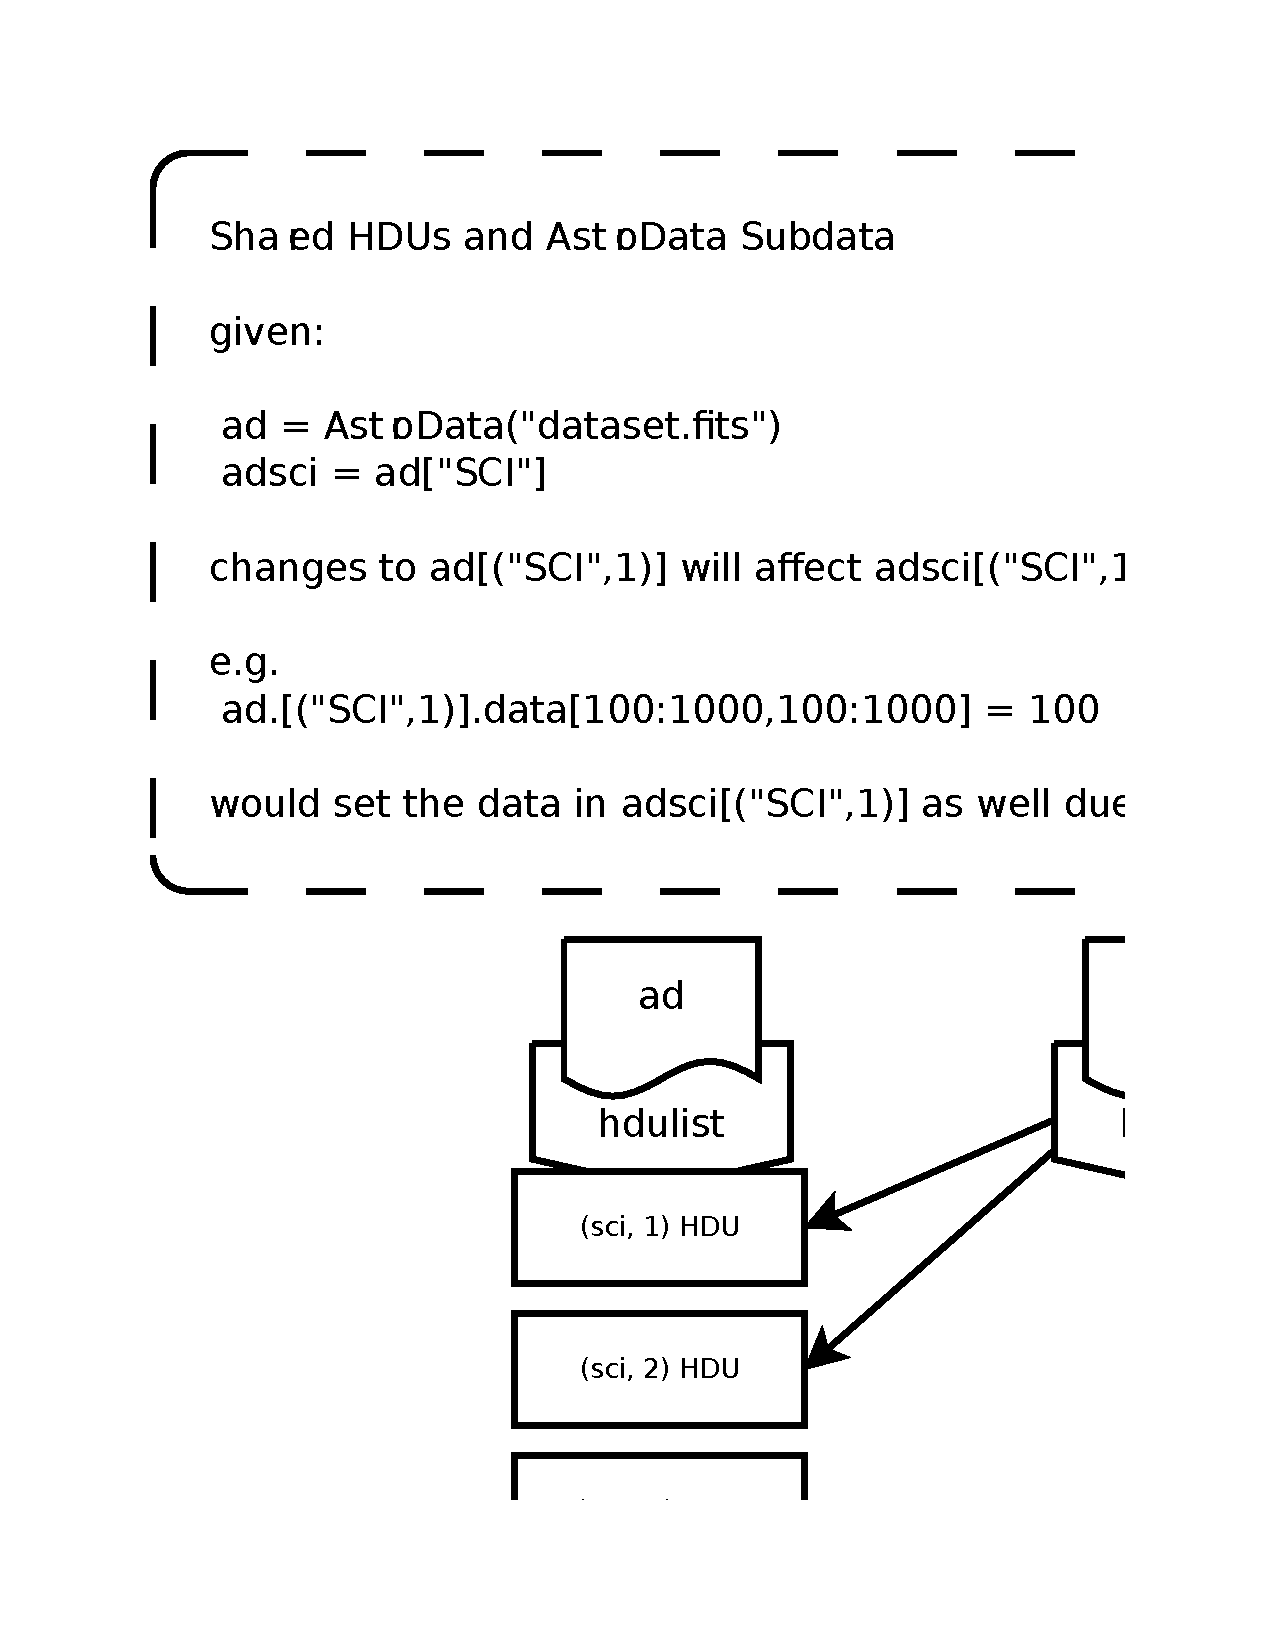
\includegraphics{sharedHDUs.pdf}}\hfill}

AstroData instances are presented as lists of AstroData instances.
However, internally the list is merely a list of extensions and the
\emph{AstroData.getitem(..)} function (which implements the ``{[}{]}'' syntax)
creates AstroData instances on the fly when called. Such instances
share information in memory with their parent instance. This is in
line with the general operation of pyfits and numpy, and in general
how Python handles objects. This allows efficient use of memory and
disk I/O. To make copies one must explicitly ask for copies. Thus when
one takes a slice of a numpy array, that slice, although possibly of a
different dimensionality and certainly of range, is really just a view
onto the original memory, changes to the slice affect the original. If
one takes a subset of an AstroData instance's HDUList, then the save
HDUs are present in both the original and the sub-data. To make a
separate copy one must use the \emph{deepcopy} built-in function (see
below).

As the diagram indicates, when taking a subset of data from an
AstroData instance using the square brackets operator, you receive a
newly created AstroData instance which is associated only with those
HDUs identified. Changes to a shared HDU's data or header member will
be reflected in both AstroData instances. Generally speaking this is
what you want for efficient operation. If you do want to have entirely
separate data, such that changes to the data sections of one do not
affect the other, use the python deepcopy operator:

\begin{Verbatim}[commandchars=\\\{\},numbers=left,firstnumber=1,stepnumber=1]
\PYG{k+kn}{from} \PYG{n+nn}{copy} \PYG{k+kn}{import} \PYG{n}{deepcopy}

\PYG{n}{ad} \PYG{o}{=} \PYG{n}{AstroData}\PYG{p}{(}\PYG{l+s}{"}\PYG{l+s}{dataset.fits}\PYG{l+s}{"}\PYG{p}{)}
\PYG{n}{scicopy} \PYG{o}{=} \PYG{n}{deepcopy}\PYG{p}{(}\PYG{n}{ad}\PYG{p}{[}\PYG{l+s}{"}\PYG{l+s}{SCI}\PYG{l+s}{"}\PYG{p}{]}\PYG{p}{)}
\end{Verbatim}

If on the other hand all you want is to avoid changing the original
dataset on disk, and do not need the original data, untransformed, in
memory along with the transformed version, which is the usual case,
then you can write the AstroData subdata instance to a new filename:

\begin{Verbatim}[commandchars=\\\{\},numbers=left,firstnumber=1,stepnumber=1]
\PYG{k+kn}{from} \PYG{n+nn}{astrodata} \PYG{k+kn}{import} \PYG{n}{AstroData}

\PYG{n}{ad} \PYG{o}{=} \PYG{n}{AstroData}\PYG{p}{(}\PYG{l+s}{"}\PYG{l+s}{dataset.fits}\PYG{l+s}{"}\PYG{p}{)}
\PYG{n}{scicopy} \PYG{o}{=} \PYG{n}{ad}\PYG{p}{[}\PYG{l+s}{"}\PYG{l+s}{SCI}\PYG{l+s}{"}\PYG{p}{]}
\PYG{n}{scicopy}\PYG{o}{.}\PYG{n}{write}\PYG{p}{(}\PYG{l+s}{"}\PYG{l+s}{datasetSCI.fits}\PYG{l+s}{"}\PYG{p}{)}
\end{Verbatim}


\subsection{count\_exts(..)}
\label{chapter_AstroDataClass:count-exts}\index{count\_exts() (astrodata.data.AstroData method)}

\begin{fulllineitems}
\phantomsection\label{chapter_AstroDataClass:astrodata.data.AstroData.count_exts}\pysiglinewithargsret{\code{AstroData.}\bfcode{count\_exts}}{\emph{extname=None}}{}~\begin{quote}\begin{description}
\item[{Parameters}] \leavevmode
\textbf{extname} (\emph{string}) -- the name of the extension, equivalent to the
value associated with the ``EXTNAME'' key in the extension 
header.

\item[{Returns}] \leavevmode
number of extensions of that name

\item[{Return type}] \leavevmode
int

\end{description}\end{quote}

The count\_exts(..) function counts the extensions of a given name
(as stored in the HDUs ``EXTNAME'' header).

\end{fulllineitems}



\subsection{The {[}{]} Operator}
\label{chapter_AstroDataClass:the-operator}\index{\_\_getitem\_\_() (astrodata.data.AstroData method)}

\begin{fulllineitems}
\phantomsection\label{chapter_AstroDataClass:astrodata.data.AstroData.__getitem__}\pysiglinewithargsret{\code{AstroData.}\bfcode{\_\_getitem\_\_}}{\emph{ext}}{}~\begin{quote}\begin{description}
\item[{Parameters}] \leavevmode
\textbf{ext} (\emph{string, int, or tuple}) -- The integer index, an indexing \code{(EXTNAME, EXTVER)} tuple,
or EXTNAME name. If an int or tuple, the single
extension identified is wrapped with an AstroData instance, and
``single-extension'' members of the AstroData object can be used. If
a string, \code{EXTNAME}, is given, then all extensions with the given 
EXTNAME will be wrapped by the  new AstroData instance.

\item[{Returns}] \leavevmode
an AstroData instance associated with the subset of data.

\item[{Return type}] \leavevmode
AstroData

\end{description}\end{quote}

This function supports the ``{[}{]}'' syntax for AstroData instances,
e.g. \emph{ad{[}(``SCI'',1){]}}.  We use it to create
AstroData objects associated with ``subdata'' of the parent
AstroData object, that is, consisting of an HDUList made up of 
some subset of the parent MEF. e.g.:

\begin{Verbatim}[commandchars=\\\{\}]
\PYG{k+kn}{from} \PYG{n+nn}{astrodata} \PYG{k+kn}{import} \PYG{n}{AstroData}

\PYG{n}{datasetA} \PYG{o}{=} \PYG{n}{AstroData}\PYG{p}{(}\PYG{l+s}{"}\PYG{l+s}{datasetMEF.fits}\PYG{l+s}{"}\PYG{p}{)}
\PYG{n}{datasetB} \PYG{o}{=} \PYG{n}{datasetA}\PYG{p}{[}\PYG{n}{SCI}\PYG{p}{]}
\end{Verbatim}

In this case, after the operations, datasetB is an \code{AstroData} object
associated with the same MEF, sharing some of the the same actual HDUs
in memory as \code{datasetA}. The object in \code{datasetB} will behave as if the
SCI extensions are its only members, and it does in fact have its own
\code{pyfits.HDUList}. Note that \code{datasetA} and \code{datasetB} share the PHU and also
the data structures of the HDUs they have in common, so that a change
to \code{datasetA{[}('SCI',1){]}.data} will change the 
\code{datasetB{[}('SCI',1){]}.data} member and vice versa. They are in fact both
references to the same \code{numpy} array in memory. The \code{HDUList} is a 
different list, however, that references common HDUs. If a subdata 
related \code{AstroData} object is written to disk, the resulting MEF will
contain only the extensions in the subdata's \code{HDUList}.
\begin{quote}\begin{description}
\item[{Note }] \leavevmode
Integer extensions start at 0 for the data-containing 
extensions, not at the PHU as with \code{pyfits}.  This is important:
\code{ad{[}0{]}} is the first content extension, in a traditional MEF 
perspective, the extension AFTER the PHU; it is not the PHU!  In
\code{AstroData} instances, the PHU is purely a header, and not counted
as an extension in the way that headers generally are not counted
as their own elements in the array they contain meta-data for.
The PHU can be accessed via the \code{phu} \code{AstroData} member of using
the PHU related member functions.

\end{description}\end{quote}

\end{fulllineitems}



\section{Single HDU AstroData Attributes}
\label{chapter_AstroDataClass:single-hdu-astrodata-attributes}

\subsection{data attribute}
\label{chapter_AstroDataClass:data-attribute}\index{data (astrodata.data.AstroData attribute)}

\begin{fulllineitems}
\phantomsection\label{chapter_AstroDataClass:astrodata.data.AstroData.data}\pysigline{\code{AstroData.}\bfcode{data}}
The data property can only be used for single-HDU AstroData
instances, such as those returned during iteration. It is a property
attribute which uses \emph{get\_data(..)} and \emph{set\_data(..)} to access the
data members with ``='' syntax. To set the data member, use \emph{ad.data =
newdata}, where \emph{newdata} must be a numpy array. To get the data
member, use \emph{npdata = ad.data}.

\end{fulllineitems}

\index{get\_data() (astrodata.data.AstroData method)}

\begin{fulllineitems}
\phantomsection\label{chapter_AstroDataClass:astrodata.data.AstroData.get_data}\pysiglinewithargsret{\code{AstroData.}\bfcode{get\_data}}{}{}~\begin{quote}\begin{description}
\item[{Returns}] \leavevmode
data array associated with the single extension

\item[{Return type}] \leavevmode
pyfits.ndarray

\end{description}\end{quote}

The \code{get\_data(..)} member is the function behind the property-style
``data'' member and returns appropriate HDU's data member(s) specifically
for the case in which the \code{AstroData} instance has ONE HDU (in addition to
the PHU). This allows a single-extension \code{AstroData}, such as \code{AstroData}
generates through iteration,  to be used as though it simply is just the
one extension, e.g. allowing \code{ad.data} to be used in place of the more
esoteric and ultimately more dangerous \code{ad{[}0{]}.data}. One
is dealing with single extension \code{AstroData} instances when iterating over
the \code{AstroData} extensions and when picking out an extension by integer
or tuple indexing, e.g.:

\begin{Verbatim}[commandchars=\\\{\}]
\PYG{k}{for} \PYG{n}{ad} \PYG{o+ow}{in} \PYG{n}{dataset}\PYG{p}{[}\PYG{n}{SCI}\PYG{p}{]}\PYG{p}{:}
    \PYG{c}{\PYGZsh{} ad is a single-HDU index}
    \PYG{n}{ad}\PYG{o}{.}\PYG{n}{data} \PYG{o}{=} \PYG{n}{newdata}

\PYG{c}{\PYGZsh{} assuming the named extension exists,}
\PYG{c}{\PYGZsh{} sd will be a single-HDU AstroData}
\PYG{n}{sd} \PYG{o}{=} \PYG{n}{dataset}\PYG{p}{[}\PYG{p}{(}\PYG{l+s}{"}\PYG{l+s}{SCI}\PYG{l+s}{"}\PYG{p}{,}\PYG{l+m+mi}{1}\PYG{p}{)}\PYG{p}{]}
\end{Verbatim}

\end{fulllineitems}

\index{set\_data() (astrodata.data.AstroData method)}

\begin{fulllineitems}
\phantomsection\label{chapter_AstroDataClass:astrodata.data.AstroData.set_data}\pysiglinewithargsret{\code{AstroData.}\bfcode{set\_data}}{\emph{newdata}}{}~\begin{quote}\begin{description}
\item[{Parameters}] \leavevmode
\textbf{newdata} (\emph{numpy.ndarray}) -- new data objects

\item[{Raises Errors.SingleHDUMemberExcept}] \leavevmode
if AstroData instance has more 
than one extension (not including PHU).

\end{description}\end{quote}

This function sets the data member of a data section of an \code{AstroData}
object, specifically for the case in which the \code{AstroData} instance has
ONE header-data unit (in addition to PHU).  This case is assured when
iterating over the \code{AstroData} extensions, as in:

\begin{Verbatim}[commandchars=\\\{\}]
\PYG{k}{for} \PYG{n}{ad} \PYG{o+ow}{in} \PYG{n}{dataset}\PYG{p}{[}\PYG{n}{SCI}\PYG{p}{]}\PYG{p}{:}
    \PYG{o}{.}\PYG{o}{.}\PYG{o}{.}
\end{Verbatim}

\end{fulllineitems}



\subsection{header attribute}
\label{chapter_AstroDataClass:header-attribute}\index{header (astrodata.data.AstroData attribute)}

\begin{fulllineitems}
\phantomsection\label{chapter_AstroDataClass:astrodata.data.AstroData.header}\pysigline{\code{AstroData.}\bfcode{header}}
The header property can only be used for single-HDU AstroData
instances, such as those returned during iteration. It is a
property attribute which uses \emph{get\_header(..)} and
\emph{set\_header(..)} to access the header member with the ``='' syntax.
To set the header member, use \emph{ad.header = newheader}, where
\emph{newheader} must be a pyfits.Header object. To get the header
member, use \emph{hduheader = ad.header}.

\end{fulllineitems}

\index{get\_header() (astrodata.data.AstroData method)}

\begin{fulllineitems}
\phantomsection\label{chapter_AstroDataClass:astrodata.data.AstroData.get_header}\pysiglinewithargsret{\code{AstroData.}\bfcode{get\_header}}{\emph{extension=None}}{}~\begin{quote}\begin{description}
\item[{Returns}] \leavevmode
header

\item[{Return type}] \leavevmode
pyfits.Header

\item[{Raises Errors.SingleHDUMemberExcept}] \leavevmode
Will raise an exception if more
than one extension exists. 
(note: The PHU is not considered an extension in this case)

\end{description}\end{quote}

The \code{get\_header(..)} function returns the header member for Single-HDU
\code{AstroData} instances (which are those that have only one extension plus
PHU). This case  can be assured when iterating over extensions using
\code{AstroData}, e.g.:

\begin{Verbatim}[commandchars=\\\{\}]
\PYG{k}{for} \PYG{n}{ad} \PYG{o+ow}{in} \PYG{n}{dataset}\PYG{p}{[}\PYG{n}{SCI}\PYG{p}{]}\PYG{p}{:} 
    \PYG{o}{.}\PYG{o}{.}\PYG{o}{.}
\end{Verbatim}

\end{fulllineitems}

\index{set\_header() (astrodata.data.AstroData method)}

\begin{fulllineitems}
\phantomsection\label{chapter_AstroDataClass:astrodata.data.AstroData.set_header}\pysiglinewithargsret{\code{AstroData.}\bfcode{set\_header}}{\emph{header}, \emph{extension=None}}{}~\begin{quote}\begin{description}
\item[{Parameters}] \leavevmode\begin{itemize}
\item {} 
\textbf{header} (\emph{pyfits.Header}) -- pyfits Header to set for given extension

\item {} 
\textbf{extension} (\emph{int or tuple, pyfits compatible extension index}) -- Extension index to retrieve header, if None
or not present then this must be a single extension AstroData
instance, which contains just the PHU and a single data extension,
and the data extension's header is returned.

\end{itemize}

\item[{Raises Errors.SingleHDUMemberExcept}] \leavevmode
Will raise an exception if more 
than one extension exists.

\end{description}\end{quote}

The \code{set\_header(..)} function sets the extension header member for single
extension (which are those that have only one extension plus PHU). This
case  is assured when iterating over extensions using \code{AstroData}, e.g.:
\begin{quote}
\begin{description}
\item[{for ad in dataset{[}SCI{]}: }] \leavevmode
...

\end{description}
\end{quote}

\end{fulllineitems}



\subsection{Renaming an Extension}
\label{chapter_AstroDataClass:renaming-an-extension}\index{rename\_ext() (astrodata.data.AstroData method)}

\begin{fulllineitems}
\phantomsection\label{chapter_AstroDataClass:astrodata.data.AstroData.rename_ext}\pysiglinewithargsret{\code{AstroData.}\bfcode{rename\_ext}}{\emph{name}, \emph{ver=None}, \emph{force=True}}{}~\begin{quote}\begin{description}
\item[{Parameters}] \leavevmode\begin{itemize}
\item {} 
\textbf{name} (\emph{string}) -- New `EXTNAME' for the given extension.

\item {} 
\textbf{ver} (\emph{int}) -- New `EXTVER' for the given extension

\item {} 
\textbf{force} (\emph{boolean}) -- ???  Default=True

\end{itemize}

\end{description}\end{quote}

Note: This member only works on single extension \code{AstroData} instances.

The \code{rename\_ext(..)} function is used in order to rename an HDU with a new
EXTNAME and EXTVER identifier.  Merely changing the EXTNAME and 
EXTEVER values in the extensions \code{pyfits.Header} are not sufficient.
Though the values change in the \code{pyfits.Header} object, there are special
HDU class members which are not updated.
\begin{quote}\begin{description}
\item[{Warning }] \leavevmode
This function manipulates private (or somewhat private)  HDU
members, specifically `name' and `\_extver'. STSCI has been
informed of the issue and
has made a special HDU function for performing the renaming. 
When generally available, this new function will be used instead of
manipulating the  HDU's properties directly, and this function will 
call the new \code{pyfits.HDUList(..)} function.

\end{description}\end{quote}

\end{fulllineitems}



\section{Module Level Functions}
\label{chapter_AstroDataClass:module-level-functions}

\subsection{correlate(..)}
\label{chapter_AstroDataClass:correlate}\index{correlate() (in module astrodata.data)}

\begin{fulllineitems}
\phantomsection\label{chapter_AstroDataClass:astrodata.data.correlate}\pysiglinewithargsret{\code{astrodata.data.}\bfcode{correlate}}{\emph{*iary}}{}~\begin{quote}\begin{description}
\item[{Parameters}] \leavevmode
\textbf{iary} (\emph{list of AstroData instance}) -- A list of AstroData instances for which a correlation dictionary
will be constructed.

\item[{Returns}] \leavevmode
a list of tuples containing correlated extensions from the arguments.

\item[{Return type}] \leavevmode
list of tuples

\end{description}\end{quote}

The \code{correlate(..)} function is a module-level helper function which returns
a list of tuples of Single Extension \code{AstroData} instances which associate
extensions from each listed AstroData object, to identically named
extensions among the rest of the input array. The \code{correlate(..)} function
accepts a variable number of arguments, all of which should be \code{AstroData}
instances.

The function returns a structured dictionary of dictionaries of lists of
\code{AstroData} objects. For example, given three inputs, \emph{ad}, \emph{bd} and \emph{cd}, all
with three ``SCI'', ``VAR'' and ``DQ'' extensions. Given \emph{adlist = {[}ad, bd,
cd{]}}, then \emph{corstruct = correlate(adlist)} will return to \emph{corstruct} a
dictionary first keyed by the EXTNAME, then keyed by tuple. The contents
(e.g. of \emph{corstruct{[}''SCI''{]}{[}1{]}}) are just a list of AstroData instances each
containing a header-data unit from \emph{ad}, \emph{bd}, and \emph{cd} respectively.
\begin{quote}\begin{description}
\item[{Info }] \leavevmode
to appear in the list, all the given arguments must have an extension
with the given (EXTNAME,EXTVER) for that tuple.

\end{description}\end{quote}

\end{fulllineitems}



\subsection{prep\_output(..)}
\label{chapter_AstroDataClass:prep-output}\index{prep\_output() (in module astrodata.data)}

\begin{fulllineitems}
\phantomsection\label{chapter_AstroDataClass:astrodata.data.prep_output}\pysiglinewithargsret{\code{astrodata.data.}\bfcode{prep\_output}}{\emph{input\_ary=None}, \emph{name=None}, \emph{clobber=False}}{}~\begin{quote}\begin{description}
\item[{Parameters}] \leavevmode\begin{itemize}
\item {} 
\textbf{input\_ary} (\emph{list of AstroData Instances}) -- The input array from which propagated content (such as
the  source PHU) will be taken. Note: the zero-th element in the list
is  used as the reference dataset for PHU or other items which require
a particular reference.

\item {} 
\textbf{name} -- File name to use for returned AstroData, optional.

\item {} 
\textbf{clobber} (\emph{bool}) -- By default \code{prep\_output(..)} checks to see if a file of the
given name already exists, and will raise an exception if found.
Set \emph{clobber} to \emph{True} to override this behavior and potentially
overwrite the extant file.  The dataset on disk will not be overwritten
as a direct result of prep\_output, which only prepares the object
in memory, but will occur when the AstroData object returned is 
written (i.e. \code{ad.write(..)})).

\end{itemize}

\item[{Returns}] \leavevmode
an \code{AstroData} instance initialized with appropriate
header-data units such as the PHU, Standard Gemini headers
and with type-specific associated  data-header units such as
binary table Mask Definition tables (MDF).

\item[{Return type}] \leavevmode
AstroData

\end{description}\end{quote}

..info: File will not have been written to disk by \code{prep\_output(..)}.

The \code{prep\_output(..)} function creates a new \code{AstroData} object ready for
appending output information (e.g. \code{ad.append(..)}).  While you can also
create an empty \code{AstroData} object by giving no arguments to the \code{AstroData}
constructor  (i.e. \code{ad = AstroData()}), \code{prep\_output(..)} exists for the
common case where a new dataset object is intended as the output of
some processing on a list of source datasets, and some information
from the source inputs must be propagated.

The \code{prep\_output(..)} function makes use of this knowledge to ensure the
file meets standards in what is considered a complete output file given
such a combination.  In the future this function can make use of dataset
history and structure definitions in the ADCONFIG configuration space. As
\code{prep\_output} improves, scripts and primitives that use it
will benefit in a forward compatible way, in that their output datasets will
benefit from more automatic propagation, validations, and data flow control,
such as the emergence of history database propagation.

Presently, it already provides the following:
\begin{itemize}
\item {} 
Ensures that all standard headers are in place in the new file, using the
configuration .

\item {} 
Copy the PHU of the reference image (\code{input\_ary{[}0{]}}).

\item {} 
Propagate associated information such as the MDF in the case of a MOS 
observation, configurable by the Astrodata Structures system.

\end{itemize}

\end{fulllineitems}



\subsection{re\_header\_keys(..)}
\label{chapter_AstroDataClass:re-header-keys}\index{re\_header\_keys() (in module astrodata.data)}

\begin{fulllineitems}
\phantomsection\label{chapter_AstroDataClass:astrodata.data.re_header_keys}\pysiglinewithargsret{\code{astrodata.data.}\bfcode{re\_header\_keys}}{\emph{rekey}, \emph{header}}{}~\begin{quote}\begin{description}
\item[{Parameters}] \leavevmode\begin{itemize}
\item {} 
\textbf{rekey} (\emph{string}) -- a regular expression to match keys in header

\item {} 
\textbf{header} (\emph{pyfits.Header}) -- a \code{pyfits.Header} object as returned by \code{ad{[}("SCI",1){]}.header}

\end{itemize}

\item[{Returns}] \leavevmode
a list of matching keys

\item[{Return type}] \leavevmode
list of strings

\end{description}\end{quote}

This utility function returns a list of keys from 
the input header that match the regular expression.

\end{fulllineitems}



\chapter{ReductionContext Class Reference}
\label{chapter_ReductionContextClass:reductioncontext-class-reference}\label{chapter_ReductionContextClass::doc}
The following is information about the ReductionContext class. When writing
primitives the reduction context is passed into the primitive as the sole
argument (generally named \code{rc} by
Gemini conventions and in addition to the \code{self} argument).
This object is used by the primitive to both get inputs
and store outputs, as well as to communicate with subsystems
like the calibration queries system or list keeping for stacking.


\section{Parameter and Dictionary Features}
\label{chapter_ReductionContextClass:parameter-and-dictionary-features}

\subsection{The ``in'' operator: contains(..)}
\label{chapter_ReductionContextClass:the-in-operator-contains}\index{\_\_contains\_\_() (astrodata.RecipeManager.ReductionContext method)}

\begin{fulllineitems}
\phantomsection\label{chapter_ReductionContextClass:astrodata.RecipeManager.ReductionContext.__contains__}\pysiglinewithargsret{\code{ReductionContext.}\bfcode{\_\_contains\_\_}}{\emph{thing}}{}~\begin{quote}\begin{description}
\item[{Parameters}] \leavevmode
\textbf{thing} (\emph{str}) -- A key to check for presence in the Reduction Context

\end{description}\end{quote}

The \code{\_\_contains\_\_} function implements the Python \code{in} operator. The 
\code{ReductionContext} is a subclass of a \code{dict}, but it also has a secondary
dict of ``local parameters'' which are available to the current primitive         only, which are also tested by the \code{\_\_contains\_\_(..)} member.
These parameters will generally be those passed in as arguments
to a primitive call from a recipe.

\end{fulllineitems}



\section{Dataset Streams: Input and Output Datasets}
\label{chapter_ReductionContextClass:dataset-streams-input-and-output-datasets}

\subsection{get\_inputs(..)}
\label{chapter_ReductionContextClass:get-inputs}\index{get\_inputs() (astrodata.RecipeManager.ReductionContext method)}

\begin{fulllineitems}
\phantomsection\label{chapter_ReductionContextClass:astrodata.RecipeManager.ReductionContext.get_inputs}\pysiglinewithargsret{\code{ReductionContext.}\bfcode{get\_inputs}}{\emph{style=None}}{}~\begin{quote}\begin{description}
\item[{Parameters}] \leavevmode
\textbf{style} (\emph{string}) -- Controls the type of return value. Supported values are ``AD''
and ``FN'' for \code{AstroData} and \code{string} filenames respectively.

\item[{Returns}] \leavevmode
a list of \code{AstroData} instances or \code{string} filenames

\item[{Return type}] \leavevmode
list

\end{description}\end{quote}

\code{get\_inputs(..)} gets the current input datasets from the current stream. You cannot
choose the stream, use \code{get\_stream(..)} for that.  To report modified
datasets back to the stream use \code{report\_output(..)}.

\end{fulllineitems}



\subsection{get\_inputs\_as\_astrodata(..)}
\label{chapter_ReductionContextClass:get-inputs-as-astrodata}\index{get\_inputs\_as\_astrodata() (astrodata.RecipeManager.ReductionContext method)}

\begin{fulllineitems}
\phantomsection\label{chapter_ReductionContextClass:astrodata.RecipeManager.ReductionContext.get_inputs_as_astrodata}\pysiglinewithargsret{\code{ReductionContext.}\bfcode{get\_inputs\_as\_astrodata}}{}{}
This function is equivalent to:

get\_inputs(style=''AD'')

\end{fulllineitems}



\subsection{get\_inputs\_as\_filenames(..)}
\label{chapter_ReductionContextClass:get-inputs-as-filenames}\index{get\_inputs\_as\_filenames() (astrodata.RecipeManager.ReductionContext method)}

\begin{fulllineitems}
\phantomsection\label{chapter_ReductionContextClass:astrodata.RecipeManager.ReductionContext.get_inputs_as_filenames}\pysiglinewithargsret{\code{ReductionContext.}\bfcode{get\_inputs\_as\_filenames}}{}{}
This function is equivalent for:

get\_inputs(style=''FN'')

\end{fulllineitems}



\subsection{get\_stream(..)}
\label{chapter_ReductionContextClass:get-stream}\index{get\_stream() (astrodata.RecipeManager.ReductionContext method)}

\begin{fulllineitems}
\phantomsection\label{chapter_ReductionContextClass:astrodata.RecipeManager.ReductionContext.get_stream}\pysiglinewithargsret{\code{ReductionContext.}\bfcode{get\_stream}}{\emph{stream='main'}, \emph{empty=False}, \emph{style=None}}{}~\begin{quote}\begin{description}
\item[{Parameters}] \leavevmode\begin{itemize}
\item {} 
\textbf{stream} (\emph{str}) -- A string name for the stream in question.  
To use the standard stream do not set.

\item {} 
\textbf{empty} (\emph{bool}) -- Controls if the stream is
emptied, defaults to ``False''.

\item {} 
\textbf{style} -- controls the type of output. ``AD'' directs the function
to return a list
of AstroData instances. ``FN'' directs it to return a list of filenames.
If left blank or set to \code{None}, the AstroDataRecord structures used
by the Reduction Context will be returned.

\end{itemize}

\item[{Returns}] \leavevmode
a list of \code{AstroDataRecord} objects, \code{AstroData} objects or filenames.

\item[{Return type}] \leavevmode
list

\end{description}\end{quote}

\code{get\_stream} returns a list of AstroData instances in the specified stream.

\end{fulllineitems}



\subsection{get\_reference\_image(..)}
\label{chapter_ReductionContextClass:get-reference-image}\index{get\_reference\_image() (astrodata.RecipeManager.ReductionContext method)}

\begin{fulllineitems}
\phantomsection\label{chapter_ReductionContextClass:astrodata.RecipeManager.ReductionContext.get_reference_image}\pysiglinewithargsret{\code{ReductionContext.}\bfcode{get\_reference\_image}}{}{}
This function returns the current reference image.  At the moment
this is simply the first dataset in the current inputs.  However,
use of this function allows us to evolve our concept of reference
image for more complicated cases where the choice of a ``reference'' image
may need to be different (e.g. require some data analysis to determine).

\end{fulllineitems}



\subsection{report\_output(..)}
\label{chapter_ReductionContextClass:report-output}\index{report\_output() (astrodata.RecipeManager.ReductionContext method)}

\begin{fulllineitems}
\phantomsection\label{chapter_ReductionContextClass:astrodata.RecipeManager.ReductionContext.report_output}\pysiglinewithargsret{\code{ReductionContext.}\bfcode{report\_output}}{\emph{inp}, \emph{stream=None}, \emph{load=True}}{}~\begin{quote}\begin{description}
\item[{Parameters}] \leavevmode\begin{itemize}
\item {} 
\textbf{inp} (\emph{str, AstroData instance, or list}) -- The inputs to report (add to the given or current stream).
Input can be a string (filename), an AstroData instance, or a list of
strings and/or AstroData instances.  Each individual dataset is
wrapped in an AstroDataRecord and stored in the current stream.

\item {} 
\textbf{stream} (\emph{str}) -- If not specified the default (``main'') stream is used.
When specified the named stream is created if necessary.

\item {} 
\textbf{load} -- A boolean (default: True) which specifies whether string
arguments (pathnames) should be loaded into AstroData instances
or if it should be kept as a filename, unloaded.  This argument
has no effect when ``report''
\code{AstroData} instances already in memory.

\end{itemize}

\end{description}\end{quote}

This function, along with \code{get\_inputs(..)} allows a primitive to
interact with the datastream in which it was invoked (or access
other streams).

\end{fulllineitems}



\subsection{switch\_stream(..)}
\label{chapter_ReductionContextClass:switch-stream}\index{switch\_stream() (astrodata.RecipeManager.ReductionContext method)}

\begin{fulllineitems}
\phantomsection\label{chapter_ReductionContextClass:astrodata.RecipeManager.ReductionContext.switch_stream}\pysiglinewithargsret{\code{ReductionContext.}\bfcode{switch\_stream}}{\emph{switch\_to=None}}{}~\begin{quote}\begin{description}
\item[{Parameters}] \leavevmode
\textbf{switch\_to} (\emph{str}) -- The string name of the stream to switch to. The 
named stream must already exist.

\item[{Note }] \leavevmode
This function is used by the infrastructure (in an application
such as reduce and in the ReductionContext) to switch the stream
being used. Reported output then goes to the specified stream.

\end{description}\end{quote}

\end{fulllineitems}



\section{ADCC Services}
\label{chapter_ReductionContextClass:adcc-services}

\section{Calibrations}
\label{chapter_ReductionContextClass:calibrations}

\subsection{get\_cal(..)}
\label{chapter_ReductionContextClass:get-cal}\index{get\_cal() (astrodata.RecipeManager.ReductionContext method)}

\begin{fulllineitems}
\phantomsection\label{chapter_ReductionContextClass:astrodata.RecipeManager.ReductionContext.get_cal}\pysiglinewithargsret{\code{ReductionContext.}\bfcode{get\_cal}}{\emph{data}, \emph{caltype}}{}
Retrieve calibration.
\begin{quote}\begin{description}
\item[{Parameters}] \leavevmode\begin{itemize}
\item {} 
\textbf{data} (\emph{string or AstroData instance}) -- File for which calibration must be retrieved.

\item {} 
\textbf{caltype} (\emph{string}) -- The type of calibration (ex.'bias', `flat').

\end{itemize}

\item[{Returns}] \leavevmode
The URI of the currently stored calibration or None.

\item[{Return type}] \leavevmode
string or None

\end{description}\end{quote}

\end{fulllineitems}



\subsection{rq\_cal(..)}
\label{chapter_ReductionContextClass:rq-cal}\index{rq\_cal() (astrodata.RecipeManager.ReductionContext method)}

\begin{fulllineitems}
\phantomsection\label{chapter_ReductionContextClass:astrodata.RecipeManager.ReductionContext.rq_cal}\pysiglinewithargsret{\code{ReductionContext.}\bfcode{rq\_cal}}{\emph{caltype}, \emph{inputs=None}, \emph{source='all'}}{}
Create calibration requests based on raw inputs.
\begin{quote}\begin{description}
\item[{Parameters}] \leavevmode\begin{itemize}
\item {} 
\textbf{caltype} (\emph{str}) -- The type of calibration. For example, `bias' and `flat'.

\item {} 
\textbf{inputs} (\emph{list of AstroData instances}) -- The datasets for which to find calibrations, if not present
or \code{None} current ``inputs'' are used.

\item {} 
\textbf{source} -- Directs what calibration service to contact, for future
compatibility, currently only ``all'' is supported.

\end{itemize}

\end{description}\end{quote}

\end{fulllineitems}



\section{Stacking}
\label{chapter_ReductionContextClass:stacking}

\subsection{rq\_stack\_get(..)}
\label{chapter_ReductionContextClass:rq-stack-get}\index{rq\_stack\_get() (astrodata.RecipeManager.ReductionContext method)}

\begin{fulllineitems}
\phantomsection\label{chapter_ReductionContextClass:astrodata.RecipeManager.ReductionContext.rq_stack_get}\pysiglinewithargsret{\code{ReductionContext.}\bfcode{rq\_stack\_get}}{\emph{purpose='`}}{}~\begin{quote}\begin{description}
\item[{Parameters}] \leavevmode
\textbf{purpose} (\emph{string}) -- The purpose is a string prepended to the stackingID
used to identify the list (see \code{get\_list(..)}).

\end{description}\end{quote}

The stackingID (see IDFactory module) is used to identify the list.
The first input in the rc.inputs list is used as the reference image 
to generate  
the stackingID portion of the list identifier.

The stackingID function in IDFactory is meant to produce identical
stacking identifiers for different images which can/should be stacked 
together, e.g. based
on program ID and/or other details.  Again, see IDFactory for the
particular algorithm in use.
\begin{quote}\begin{description}
\item[{Note }] \leavevmode
a versioning system is latent within the code, and is added
to the id to allow adaptation in the future if identifer construction
methods change.

\end{description}\end{quote}

\end{fulllineitems}



\subsection{rq\_stack\_update(..)}
\label{chapter_ReductionContextClass:rq-stack-update}\index{rq\_stack\_update() (astrodata.RecipeManager.ReductionContext method)}

\begin{fulllineitems}
\phantomsection\label{chapter_ReductionContextClass:astrodata.RecipeManager.ReductionContext.rq_stack_update}\pysiglinewithargsret{\code{ReductionContext.}\bfcode{rq\_stack\_update}}{\emph{purpose=None}}{}~\begin{quote}\begin{description}
\item[{Parameters}] \leavevmode
\textbf{purpose} (\emph{str}) -- The purpose argument is a string prefixed to the
generated stackingID.  This allows two images which would
produce identical stackingIDs to go in different lists,
i.e. such as a fringe frame which might be prepended with
``fringe'' as the purpose.

\end{description}\end{quote}

This function creates requests to update a stack list with the files
in the current rc.inputs list.  Each will go in a stack based on its
own stackingID (prepended with ``purpose'').
\begin{quote}\begin{description}
\item[{Note }] \leavevmode
this function places a message on an outbound message queue
which will not be sent until the next ``yield'', allowing the
ReductionObject command clause to execute.

\end{description}\end{quote}

\end{fulllineitems}



\section{Lists}
\label{chapter_ReductionContextClass:lists}

\subsection{list\_append(..)}
\label{chapter_ReductionContextClass:list-append}\index{list\_append() (astrodata.RecipeManager.ReductionContext method)}

\begin{fulllineitems}
\phantomsection\label{chapter_ReductionContextClass:astrodata.RecipeManager.ReductionContext.list_append}\pysiglinewithargsret{\code{ReductionContext.}\bfcode{list\_append}}{\emph{id}, \emph{files}, \emph{cachefile=None}}{}~\begin{quote}\begin{description}
\item[{Parameters}] \leavevmode\begin{itemize}
\item {} 
\textbf{id} (\emph{string}) -- A string that identifies to which list to append the filenames.

\item {} 
\textbf{files} (\emph{list of strings}) -- A list of filenames to add to the list.

\item {} 
\textbf{cachefile} (\emph{string}) -- Filename to use to store the list.

\end{itemize}

\end{description}\end{quote}

The caller is expected to supply \code{cachefile}, which in principle
a value of ``None'' could mean the ``default cachefile'' this is not
supported by the \code{adcc} as of yet. The desired behavior is for
reduce instances running in the same directory to cooperate, and those
running in separate directories be kept separate, and this is 
implemented by providing an argument for \code{cachefile} which is in a 
generated subdirectory (hidden) based on the startup directory
for the reduce process.

The adcc will negotiate all contention and race conditions regarding
multiple applications manipulating a list simultaneously in separate
process.

\end{fulllineitems}



\subsection{get\_list(..)}
\label{chapter_ReductionContextClass:get-list}\index{get\_list() (astrodata.RecipeManager.ReductionContext method)}

\begin{fulllineitems}
\phantomsection\label{chapter_ReductionContextClass:astrodata.RecipeManager.ReductionContext.get_list}\pysiglinewithargsret{\code{ReductionContext.}\bfcode{get\_list}}{\emph{id}}{}~\begin{quote}\begin{description}
\item[{Parameters}] \leavevmode
\textbf{id} (\emph{str}) -- Lists are associated with arbitrary identifiers,
passed as strings.  See \code{IDFactory} for IDs built from
standard \code{astrodata} characteristics.

\end{description}\end{quote}

The list functionality allows storing dataset names in a list
which is shared by all instances of reduce running in a given
directory.  The list is kept by an \code{adcc} instance in charge of that
sub-directory.  The \code{get\_list(..)} function retrieves a list that has
already been requested via \code{rq\_stack\_get(..)} which initiates the
interprocess request.

This function does not block, and if the stack was not requested
prior to a yeild, prior to this call, then None or an out of date
version of this list will be retrieved.
\begin{quote}\begin{description}
\item[{Note }] \leavevmode
``get\_stack'' calls get\_list but takes a ``purpose'' to which it adds
a stackingID as a suffix to the list identifier.

\end{description}\end{quote}

\end{fulllineitems}



\section{Utility}
\label{chapter_ReductionContextClass:utility}

\subsection{prepend\_names(..)}
\label{chapter_ReductionContextClass:prepend-names}\index{prepend\_names() (astrodata.RecipeManager.ReductionContext method)}

\begin{fulllineitems}
\phantomsection\label{chapter_ReductionContextClass:astrodata.RecipeManager.ReductionContext.prepend_names}\pysiglinewithargsret{\code{ReductionContext.}\bfcode{prepend\_names}}{\emph{prepend}, \emph{current\_dir=True}, \emph{filepaths=None}}{}~\begin{quote}\begin{description}
\item[{Parameters}] \leavevmode\begin{itemize}
\item {} 
\textbf{prepend} (\emph{string}) -- The string to be put at the front of the file.

\item {} 
\textbf{current\_dir} (\emph{boolean}) -- Used if the filename (astrodata filename) is in the
current working directory.

\item {} 
\textbf{filepaths} -- If present, these file paths will be modified, otherwise
the current inputs are modified.

\end{itemize}

\item[{Returns}] \leavevmode
List of new prepended paths.

\item[{Return type}] \leavevmode
list

\end{description}\end{quote}

Prepends a prefix string to either the inputs or the given list of filenames.

\end{fulllineitems}



\subsection{run(..)}
\label{chapter_ReductionContextClass:run}\index{run() (astrodata.RecipeManager.ReductionContext method)}

\begin{fulllineitems}
\phantomsection\label{chapter_ReductionContextClass:astrodata.RecipeManager.ReductionContext.run}\pysiglinewithargsret{\code{ReductionContext.}\bfcode{run}}{\emph{stepname}}{}~\begin{quote}\begin{description}
\item[{Parameters}] \leavevmode
\textbf{stepname} -- The primitive or recipe name to run. Note: this is

\end{description}\end{quote}
\begin{description}
\item[{actually compiled as a recipe. Proxy recipe names may appear}] \leavevmode
in the logs.

\end{description}
\begin{quote}\begin{description}
\end{description}\end{quote}

The \code{run(..)} function allows a primitive to use the reduction
context to execute another recipe or primitive.

\end{fulllineitems}



\chapter{AstroData Configuration Package Development Guide}
\label{developmentGuide:astrodata-configuration-package-development-guide}\label{developmentGuide::doc}

\section{Elements}
\label{configElements:elements}\label{configElements::doc}
Instrument-mode specific behaviors available through the \code{AstroData} class
are not implemented in the \code{astrodata} package itself, but are instead loaded from
configuration packages. In the case of Gemini data the
configuration package is a directory named \code{astrodata\_Gemini}.  This
configuration path is found by astrodata by the containing directory
appearing either on the \code{PYTHONPATH}, or on either of two astrodata environment
variables, \code{RECIPEPATH} or \code{ADCONFIGPATH}.

The \code{astrodata} package searches for all directories named \code{astrodata\_\textless{}anything\textgreater{}}
in these environment variables.  Though the configurations contain
executable python, it is not meant to be imported as a regular python module but
is loaded by the astrodata package.


\subsection{The General Configuration Creation Process}
\label{configElements:the-general-configuration-creation-process}\begin{enumerate}
\item {} 
Define a tree of \code{AstroDataTypes} identifying types of your data.

\item {} 
Create ``descriptor'' functions which calculate a particular metadata
value for nodes of the \code{AstroDataType} tree defined,
such as \code{gain} or \code{filter\_name}.

\item {} 
Write Python member functions bundled into \code{PrimitivesSet} classes,
which specifically understand your dataset.

\item {} 
Assemble primitives into sequential lists, which we call  processing
``recipes''.

\end{enumerate}

Initially you will develop classifications
for your data, and functions which will provide standard information, allowing
you to use AstroData, e.g. in processing scripts.  Then you will put your
processing scripts in the form of ``primitives'' and collect these in ``recipes''
so they can be used for automated data reduction.


\subsection{Configuration Elements Which Have To Be  Developed}
\label{configElements:configuration-elements-which-have-to-be-developed}\begin{enumerate}
\item {} 
\textbf{AstroData Types} identify classifications of MEF datasets to which other
features can be assigned. Types have requirements which must hold for
an identified dataset and also information about the place of the type in
an overall type hierarchy (e.g. The GMOS type is the parent of GMOS\_IMAGE).

\item {} 
\textbf{AstroData Descriptors} are functions which calculate a particular type
of metadata which is expected to be available for all datasets throughout
the type hierarchy. Examples from the Gemini configuration package are \code{gain}
and \code{filtername}.  Different instruments
store information about the gain in unique headers, and may even require
lookup tables not located in the dataset.  Descriptors are type-appropriate
functions assigned at runtime to the astrodata instance, allowing
type-specific implementations to manage these peculiarities.

\item {} 
\textbf{Primitives} are dataset transformations meant to run in the Recipe System.
Primitives are implemented as python generator functions in sets of primitives
that apply to a common AstroDataType.

\item {} 
\textbf{Recipes} are lists of primitives stored in plain text which can be executed
by the AstroData Recipe System. While primitives work on the \code{Reduction
Context} explicitly, the reduction context is implicit in recipes
so that recipes can arguably be considered to contain
``scientifically meaningful'' steps with no ``software artifacts''.

\end{enumerate}


\section{Creating A Configuration Package}
\label{startingTheConfig:creating-a-configuration-package}\label{startingTheConfig::doc}

\subsection{Preparation}
\label{startingTheConfig:preparation}
For this work it is required that the Gemini Python AstroData package already
be installed and
functional. In general the Gemini AstroData configuration package(s) will
already
be installed somewhere on the PYTHONPATH, and Gemini Python scripts such
as \code{reduce} and
\code{typewalk} will be on the system path.  Installations from SVN will
require that the \code{astrodata/scripts} package directory be added to the PATH.


\subsection{Clone the Sample Package}
\label{startingTheConfig:clone-the-sample-package}
The easiest, and recommended way to start a new configuration package is by copying the
\code{astrodata\_Sample} package. The sample configuration package is located in
\code{astrodata/sample/astrodata\_Sample}. Copy this directory to a development workspace
as in the following example, where \code{\textless{}ad\_install\_dir\textgreater{}} should be the directory in
which the \code{astrodata} package is installed:

\begin{Verbatim}[commandchars=\\\{\}]
cd /home/username
mkdir workspace
cd workspace

cp -r \textless{}ad\_install\_dir\textgreater{}/astrodata/samples/astrodata\_Sample .
\end{Verbatim}

Note that \code{\textless{}ad\_install\_dir\textgreater{}} should already be on the \code{PYTHONPATH}.

The name of the destination can, of course, be other than \code{astrodata\_Sample},
and it can be changed later as well. For a real package it must be changed, and
though not strictly necessary, the \code{ADCONFIG\_Sample} and \code{RECIPES\_Sample} should
have ``Sample'' changed to something unique which matches the parent
\code{astrodata\_\textless{}whatever\textgreater{}} directory. So long as the \code{ADCONFIG\_} and \code{RECIPIES\_}
portion of the name is present no other aspect of the configuration will have to
change. However, every configuration package wherever on the
path must have a unique name.

You must also ensure that the new directory \emph{containing}
\code{astrodata\_Sample} is in either ADCONFIGPATH or RECIPEPATH, or alternately
for convenience (i.e. when installing packages via setup.py) in the PYTHONPATH.
If you are following the above steps, you are in the directory to which
\code{astrodata\_Sample} was copied. Add this directory to the RECIPEPATH so your copy
of \code{astrodata\_Sample} can be found:

\begin{Verbatim}[commandchars=\\\{\}]
export RECIPEPATH=\$(pwd):\$RECIPEPATH
\end{Verbatim}

You can now test that \code{astrodata\_Sample} is being
discovered by the astrodata package
by running a tool from the \code{astrodata/scripts} directory which should
have been installed to system bin directories by the \code{setup.py} process.

Assuming that you are working in the test data directory, with a subdirectory
named \code{source\_data} into which you have copied at least one fits file.
For these examples, we assume for convienience your file is named \code{test.fits}:

\begin{Verbatim}[commandchars=\\\{\}]
cd \textasciitilde{}
mkdir test\_data
cd test\_data
mkdir source\_data
cp \textless{}somepath\textgreater{}/test.fits source\_data
\end{Verbatim}

We'll assume you are working in this directory for the rest of the example.
To see if the types from \code{astrodata\_Sample} are discovered, type:

\begin{Verbatim}[commandchars=\\\{\}]
\PYG{n}{typewalk} \PYG{o}{-}\PYG{n}{c}
\end{Verbatim}

This will generate output like the following:

\begin{Verbatim}[commandchars=\\\{\}]
directory: . (/home/dpd/test\_data)
 test.fits ......................... (CAL) (GEMINI) (GEMINI\_NORTH) (GMOS)
 ................................... (GMOS\_CAL) (GMOS\_IMAGE)
 ................................... (GMOS\_IMAGE\_FLAT) (GMOS\_N) (GMOS\_RAW)
 ................................... (IMAGE) (MARKED) (OBSERVED) (RAW)
 ................................... (UNPREPARED)
\end{Verbatim}

A line should show up for \code{test.fits} and any other fits files in the current
directory \textbf{and} any subdirectory listing the AstroData types which apply to the
dataset. The list will contain some Gemini types, such as RAW and
UNPREPARED, and if the data in question is Gemini data, types associated with
the instrument-mode and processing status.

However, it should also include two types from the sample configuration,
\code{UNMARKED} (or possibly \code{MARKED} if the
dataset has been manipulated by the Sample package previously), and \code{OBSERVED}.


\section{Creating An AstroDataType}
\label{creatingAnAstroDataType:creating-an-astrodatatype}\label{creatingAnAstroDataType::doc}

\subsection{Overview}
\label{creatingAnAstroDataType:overview}
AstroData types are defined in Python classes located in either of two path
locations in the configuration package:

\begin{Verbatim}[commandchars=\\\{\}]
* {}`{}`astrodata\_Sample/classification/types{}`{}` - for typological types
* {}`{}`astrodata\_Sample/classification/status{}`{}` - for types related to processing status.
\end{Verbatim}

The type definition syntax is equivalent in both cases,
the distinction is only for organization between two
sorts of dataset classfication:
\begin{enumerate}
\item {} 
Classifications that characterize instrument-modes or generic \emph{types}
of dataset.

\item {} 
Classifications that characterize the processing state of data.

\end{enumerate}

For example, from the \code{astrodata\_Gemini} configuration, the \code{RAW} and
\code{PREPARED} are ``processing types'' in \code{astrodata\_Gemini/status/...}, whereas
\code{NICI}, \code{GMOS} and \code{GMOS\_IMAGE} are ``typological types'' located in the
\code{astrodata\_Gemini/status/...} subdirectory directory.

Since we don't know anything about the instrument or mode that this  custom package is
being developed for, the sample package will add some somewhat artificial example types
as processing types,  provided as examples in the sample package that will demonstrate
the point in general. For more complicated examples of type requirements, we'll
use examples from \code{astrodata\_Gemini}..


\subsection{The Class Definition Line by Line}
\label{creatingAnAstroDataType:the-class-definition-line-by-line}
To inspect the types in the custom package change
directory to \code{astrodata\_Sample/classifications/status} and get a directory
listing:

\begin{Verbatim}[commandchars=\\\{\}]
cd \textless{}base\_path\textgreater{}/astrodata\_Sample/classifications/status
cat adtype.UNMARKED.py
\end{Verbatim}

The contents of the file should be as below:

\begin{Verbatim}[commandchars=\\\{\},numbers=left,firstnumber=1,stepnumber=1]
 \PYG{k}{class} \PYG{n+nc}{UNMARKED}\PYG{p}{(}\PYG{n}{DataClassification}\PYG{p}{)}\PYG{p}{:}
     \PYG{n}{name}\PYG{o}{=}\PYG{l+s}{"}\PYG{l+s}{UNMARKED}\PYG{l+s}{"}
     \PYG{n}{usage} \PYG{o}{=} \PYG{l+s}{"}\PYG{l+s}{Processing Type for data not yet }\PYG{l+s}{'}\PYG{l+s}{marked}\PYG{l+s}{'}\PYG{l+s}{.}\PYG{l+s}{"}
     \PYG{n}{parent} \PYG{o}{=} \PYG{l+s}{"}\PYG{l+s}{OBSERVED}\PYG{l+s}{"}
     \PYG{n}{requirement} \PYG{o}{=} \PYG{n}{PHU}\PYG{p}{(}\PYG{p}{\PYGZob{}}\PYG{l+s}{"}\PYG{l+s}{\PYGZob{}prohibit\PYGZcb{}THEMARK}\PYG{l+s}{"}\PYG{p}{:}\PYG{l+s}{'}\PYG{l+s}{.*}\PYG{l+s}{'}\PYG{p}{\PYGZcb{}}\PYG{p}{)}

 \PYG{n}{newtypes}\PYG{o}{.}\PYG{n}{append}\PYG{p}{(}\PYG{n}{UNMARKED}\PYG{p}{(}\PYG{p}{)}\PYG{p}{)}
\end{Verbatim}

Note that type source files are read into memory and executed in a prepared environment. Thus
there is no need to import
the \code{DataClassification} class from the particular astrodata module,
this standard base class is already in
scope.

The two elements are the class itself and the \code{newtypes.append(UNMARKED())} line
which instantiates an object of the class and appends it to a list that the
ClassificationLibrary can use to inspect datasets. The ClassificationLibrary uses the
\code{newtypes} list to recieve types defined in the module, allowing multiple types to be
added to this list in a single type module if desired. At Gemini we have decided to
have just one type definition per python type file.
\begin{enumerate}
\item {} 
\code{class UNMARKED(DataClassification)}:
By convention, we name the class identically to the chosen string name, in
this case \code{UNMARKED}, however this is not required by the system.

\item {} 
\code{name="UNMARKED"}:
The classification \code{name} property stores the string used by the system
to identify the type. NOTE: when using type functionality, the user never
sees the classification object, and deals with types as strings.

\item {} 
\code{usage="Processing Type for data not yet 'marked'."}:
This is used for automatically generated documentation.

\item {} 
\code{parent="OBSERVED"}:
This is the type name of a parent class.  Note, the type need not also be
recognizes as the parent type.  The parent member is used to determine
overriding assignments in the type tree such that, of course, leaf nodes
override root nodes, e.g. for descriptor calculator and primitive set
assignments.

\item {} 
\code{requirement = PHU(\{"\{prohibit\}THEMARK":'.*'\})}:
The requirement member uses requirement classes (see below) to define the given type.
In this case, this is a PHU check to ensure that the header keyword ``THEMARK'' is not set at all
in the PHU.

\item {} 
\code{newtypes.append(UNMARKED())}:
This line appends an object instance of the new class to a pre-defined
\code{newtypes} array variable. Note, this name is the \textbf{class name} from line
1, not the type name, though by convention in Gemini AstroData Types we use
the type name as the class name.

\end{enumerate}


\subsection{The Requirement Classes}
\label{creatingAnAstroDataType:the-requirement-classes}
The requirement member of a type classification is intended to be declared
with an expression built from requirement classes.  Again, the type definition
is evaluated in a controlled environment and these classes, as well as aliases
for convienience, are already in scope.


\subsubsection{Concrete Requirements}
\label{creatingAnAstroDataType:concrete-requirements}
Concrete Requirements are those that make actual physical checks of dataset characteristics.

\begin{tabulary}{\linewidth}{|L|L|L|}
\hline
\textbf{
Requirement Type
} & \textbf{
Alias
} & \textbf{
Description
}\\\hline

ClassReq
 & 
ISCLASS
 & 
For ensuring this type is also some other
classification
\\\hline

PhuReq
 & 
PHU
 & 
Checks a PHU key/value header against a regular
expression.
\\\hline
\end{tabulary}


Object Oriented design enables us to extend requirement class ability and/or create new
requirements.  Examples: the current PHU requirement checks values only against
regular expressions, it could be expanded to make numerical comparisons (e.g. to
have a dataset type dependent on seeing thresholds). Another example that we
anticipate needing is a requirement class that checkes header values in extensions.

Currently all type checking resolves to PHU checks, see below for
a description of the PHU requirement object.


\paragraph{ISCLASS(other\_class\_name)}
\label{creatingAnAstroDataType:isclass-other-class-name}
The ISCLASS requirement accepts a string name and will cause the classification to check
if the other type applies.  Circular definitions are possible and the configuration author
must ensure such do not exist.

ISCLASS example:

\begin{Verbatim}[commandchars=\\\{\}]
\PYG{k}{class} \PYG{n+nc}{GMOS}\PYG{p}{(}\PYG{n}{DataClassification}\PYG{p}{)}\PYG{p}{:}
    \PYG{n}{name}\PYG{o}{=}\PYG{l+s}{"}\PYG{l+s}{GMOS}\PYG{l+s}{"}
    \PYG{n}{usage} \PYG{o}{=} \PYG{l+s}{'''}
\PYG{l+s}{        Applies to all data from either GMOS-North or GMOS-South instruments in any mode.}
\PYG{l+s}{        }\PYG{l+s}{'''}
    \PYG{n}{parent} \PYG{o}{=} \PYG{l+s}{"}\PYG{l+s}{GEMINI}\PYG{l+s}{"}
    \PYG{n}{requirement} \PYG{o}{=} \PYG{n}{ISCLASS}\PYG{p}{(}\PYG{l+s}{"}\PYG{l+s}{GMOS\PYGZus{}N}\PYG{l+s}{"}\PYG{p}{)} \PYG{o}{\textbar{}} \PYG{n}{ISCLASS}\PYG{p}{(}\PYG{l+s}{"}\PYG{l+s}{GMOS\PYGZus{}S}\PYG{l+s}{"}\PYG{p}{)}

    \PYG{c}{\PYGZsh{} equivalent to...}
    \PYG{c}{\PYGZsh{}   requirement = OR(}
    \PYG{c}{\PYGZsh{}                    ClassReq("GMOS\PYGZus{}N"),}
    \PYG{c}{\PYGZsh{}                    ClassReq("GMOS\PYGZus{}S")}
    \PYG{c}{\PYGZsh{}                   )}

\PYG{n}{newtypes}\PYG{o}{.}\PYG{n}{append}\PYG{p}{(} \PYG{n}{GMOS}\PYG{p}{(}\PYG{p}{)}\PYG{p}{)}
\end{Verbatim}

Since there are in fact two GMOS instruments at Gemini, one in Hawaii, one in Chile, the GMOS
type really means checking that one of these two instruments was used.

\begin{notice}{note}{Note:}
This is also an example of use of the OR requirement, and specifically a convenience
feature allowing the ``\textbar{}'' symbol to be used for pair-wise or-ing. The included comment
shows another form using the OR object constructor
which allows more than two operands to be listed.
\end{notice}


\paragraph{PHU(keyname=re\_val, {[}keyname2=re\_val2 {[}...{]}{]})}
\label{creatingAnAstroDataType:phu-keyname-re-val-keyname2-re-val2}
The PHU requirement accepts any number of arguments.  Each argument name  is used as
the PHU key name, and the value is a regular expression against which the header
value will be compared.

An example:

\begin{Verbatim}[commandchars=\\\{\}]
\PYG{k}{class} \PYG{n+nc}{GMOS\PYGZus{}NODANDSHUFFLE}\PYG{p}{(}\PYG{n}{DataClassification}\PYG{p}{)}\PYG{p}{:}
    \PYG{n}{name}\PYG{o}{=}\PYG{l+s}{"}\PYG{l+s}{GMOS\PYGZus{}NODANDSHUFFLE}\PYG{l+s}{"}
    \PYG{n}{usage} \PYG{o}{=} \PYG{l+s}{"}\PYG{l+s}{Applies to data from a GMOS instrument in Nod-And-Shuffle mode}\PYG{l+s}{"}
    \PYG{n}{parent} \PYG{o}{=} \PYG{l+s}{"}\PYG{l+s}{GMOS}\PYG{l+s}{"}
    \PYG{n}{requirement} \PYG{o}{=} \PYG{n}{PHU}\PYG{p}{(}\PYG{n}{NODPIX}\PYG{o}{=}\PYG{l+s}{'}\PYG{l+s}{.*}\PYG{l+s}{'}\PYG{p}{)}

\PYG{n}{newtypes}\PYG{o}{.}\PYG{n}{append}\PYG{p}{(}\PYG{n}{GMOS\PYGZus{}NODANDSHUFFLE}\PYG{p}{(}\PYG{p}{)}\PYG{p}{)}
\end{Verbatim}

It is also possible to prohibit a match, and to use regular expressions for key matching using a
special syntax for the key name. This is done by prepending an instruction to the key name,
but also requires passing arguments to the PHU object constructor in a different way. For
example the following requirement checks to ensure that the PHU key \code{MASKNAME} \emph{does not}
match \code{"IFU*"}:

\begin{Verbatim}[commandchars=\\\{\}]
\PYG{n}{PHU}\PYG{p}{(}\PYG{p}{\PYGZob{}}\PYG{l+s}{"}\PYG{l+s}{\PYGZob{}prohibit\PYGZcb{}MASKNAME}\PYG{l+s}{"}\PYG{p}{:} \PYG{l+s}{"}\PYG{l+s}{IFU*}\PYG{l+s}{"}\PYG{p}{\PYGZcb{}}\PYG{p}{)}
\end{Verbatim}

Note that in this case the arguments are passed to the PHU object constructor as a dictionary.
The keys in the dictionary are used to match PHU keys, and the values are regular expressions
which will be compared to PHU values.

Generally, Python helps instantiating the PHU object by turning the constructor parameter
names and their settings into the keys and values of the dictionary it uses internally.
However, Python does not like special characters like ``\{'' in argument names, so to use the
extended key syntax requires passing the dictionary.

To use regular expressions in key names (which is also considered dangerous and prone to
inefficiency), use the following syntax:

\begin{Verbatim}[commandchars=\\\{\}]
\PYG{k}{class} \PYG{n+nc}{PREPARED}\PYG{p}{(}\PYG{n}{DataClassification}\PYG{p}{)}\PYG{p}{:}

    \PYG{n}{name}\PYG{o}{=}\PYG{l+s}{"}\PYG{l+s}{PREPARED}\PYG{l+s}{"}
    \PYG{n}{usage} \PYG{o}{=} \PYG{l+s}{'}\PYG{l+s}{Applies to all }\PYG{l+s}{"}\PYG{l+s}{prepared}\PYG{l+s}{"}\PYG{l+s}{ data.}\PYG{l+s}{'}
    \PYG{n}{parent} \PYG{o}{=} \PYG{l+s}{"}\PYG{l+s}{UNPREPARED}\PYG{l+s}{"}
    \PYG{n}{requirement} \PYG{o}{=} \PYG{n}{PHU}\PYG{p}{(} \PYG{p}{\PYGZob{}}\PYG{l+s}{'}\PYG{l+s}{\PYGZob{}re\PYGZcb{}.*?PREPARE}\PYG{l+s}{'}\PYG{p}{:} \PYG{l+s}{"}\PYG{l+s}{.*?}\PYG{l+s}{"} \PYG{p}{\PYGZcb{}}\PYG{p}{)}

\PYG{n}{newtypes}\PYG{o}{.}\PYG{n}{append}\PYG{p}{(}\PYG{n}{PREPARED}\PYG{p}{(}\PYG{p}{)}\PYG{p}{)}
\end{Verbatim}

Due to our legacy reduction software conventions, Gemini datasets which have been run
through the system will have a keyword of the sort ``\textless{}x\textgreater{}PREPARE'' with a value set to a
time stamp.  The need for caution is due to, one, efficiency, since the classification
must cycle through all headers to see if the regular expression matches, and two, this
technique is prone to a name collision, i.e. in our example above... if a PHU
happens to have a key matching \code{"*PREPARE"} for some other reason than having been
processed by the Gemini Package.

Please use this feature with caution.


\subsubsection{Logical Requirement Classes}
\label{creatingAnAstroDataType:logical-requirement-classes}
The logical requirement classes use OO design to behave like requirement operators,
returning true or false based on a combination of requirements given as arguments.

\begin{tabulary}{\linewidth}{|L|L|L|}
\hline
\textbf{
Requirement Type
} & \textbf{
Alias
} & \textbf{
Description
}\\\hline

AndReq
 & 
AND
 & 
For comparing two other requirements with a logical
\code{and}
\\\hline

NotReq
 & 
NOT
 & 
For negating the truth value of another requirement
\\\hline

OrReq
 & 
OR
 & 
For comparing two other requirements with a logical
\code{or}
\\\hline
\end{tabulary}



\paragraph{AND(\textless{}requirement\textgreater{},\textless{}requirement\textgreater{} {[}, \textless{}requirement\textgreater{} {[}, \textless{}requirement\textgreater{} {]} .. {]})}
\label{creatingAnAstroDataType:and-requirement-requirement-requirement-requirement}
The AND requirement accepts other requirements as arguments. At least two arguments are needed
for the AND to be sensible, but if more are present they are also checked for truth value.

It is possible also to use the ``\&'' operator as a logical ``and'':

\begin{Verbatim}[commandchars=\\\{\}]
\PYG{n}{requirement} \PYG{o}{=} \PYG{n}{AND}\PYG{p}{(}\PYG{n}{PHU}\PYG{p}{(}\PYG{l+s}{"}\PYG{l+s}{key1}\PYG{l+s}{"}\PYG{p}{,} \PYG{l+s}{"}\PYG{l+s}{val1}\PYG{l+s}{"}\PYG{p}{)}\PYG{p}{,} \PYG{n}{PHU}\PYG{p}{(}\PYG{l+s}{"}\PYG{l+s}{key2}\PYG{l+s}{"}\PYG{p}{,} \PYG{l+s}{"}\PYG{l+s}{val2}\PYG{l+s}{"}\PYG{p}{)}\PYG{p}{)}
\end{Verbatim}

...is equivalent to:

\begin{Verbatim}[commandchars=\\\{\}]
\PYG{n}{requirement} \PYG{o}{=} \PYG{n}{PHU}\PYG{p}{(}\PYG{l+s}{"}\PYG{l+s}{key1}\PYG{l+s}{"}\PYG{p}{,} \PYG{l+s}{"}\PYG{l+s}{val1}\PYG{l+s}{"}\PYG{p}{)} \PYG{o}{\&} \PYG{n}{PHU}\PYG{p}{(}\PYG{l+s}{"}\PYG{l+s}{key2}\PYG{l+s}{"}\PYG{p}{,} \PYG{l+s}{"}\PYG{l+s}{val2}\PYG{l+s}{"}\PYG{p}{)}
\end{Verbatim}


\paragraph{NOT(\textless{}requirement\textgreater{})}
\label{creatingAnAstroDataType:not-requirement}
The NOT requirement accepts a single other requirement as arguments.
``NOT'' is used to negate some requirement. For example at Gemini we
do not view a GMOS\_BIAS as a
GMOS\_IMAGE, but it does satisfy the requirements of GMOS\_IMAGE. The need
for a separate type is due to the fact that GMOS\_IMAGE and GMOS\_BIAS require
different automated reduction (e.g. in a pipeline deployment). To accomplish
this we add a \code{NOT} requirement to GMOS\_IMAGE:

\begin{Verbatim}[commandchars=\\\{\}]
\PYG{k}{class} \PYG{n+nc}{GMOS\PYGZus{}IMAGE}\PYG{p}{(}\PYG{n}{DataClassification}\PYG{p}{)}\PYG{p}{:}
    \PYG{n}{name}\PYG{o}{=}\PYG{l+s}{"}\PYG{l+s}{GMOS\PYGZus{}IMAGE}\PYG{l+s}{"}
    \PYG{n}{usage} \PYG{o}{=} \PYG{l+s}{"""}
\PYG{l+s}{        Applies to all imaging datasets from the GMOS instruments}
\PYG{l+s}{        }\PYG{l+s}{"""}
    \PYG{n}{parent} \PYG{o}{=} \PYG{l+s}{"}\PYG{l+s}{GMOS}\PYG{l+s}{"}
    \PYG{n}{requirement} \PYG{o}{=} \PYG{n}{AND}\PYG{p}{(}\PYG{p}{[}  \PYG{n}{ISCLASS}\PYG{p}{(}\PYG{l+s}{"}\PYG{l+s}{GMOS}\PYG{l+s}{"}\PYG{p}{)}\PYG{p}{,}
                         \PYG{n}{PHU}\PYG{p}{(}\PYG{n}{GRATING}\PYG{o}{=}\PYG{l+s}{"}\PYG{l+s}{MIRROR}\PYG{l+s}{"}\PYG{p}{)}\PYG{p}{,}
                         \PYG{n}{NOT}\PYG{p}{(}\PYG{n}{ISCLASS}\PYG{p}{(}\PYG{l+s}{"}\PYG{l+s}{GMOS\PYGZus{}BIAS}\PYG{l+s}{"}\PYG{p}{)}\PYG{p}{)}  \PYG{p}{]}\PYG{p}{)}

\PYG{n}{newtypes}\PYG{o}{.}\PYG{n}{append}\PYG{p}{(}\PYG{n}{GMOS\PYGZus{}IMAGE}\PYG{p}{(}\PYG{p}{)}\PYG{p}{)}
\end{Verbatim}


\paragraph{OR(\textless{}requirement\textgreater{},\textless{}requirement\textgreater{} {[}, \textless{}requirement\textgreater{} {[}, \textless{}requirement\textgreater{} {]} .. {]})}
\label{creatingAnAstroDataType:or-requirement-requirement-requirement-requirement}
The OR requirement accepts other requirements as arguments. At least two arguments are needed
for the OR to be sensible, but if more are present they are also checked for truth value.

It is possible also to use the ``\textbar{}'' operator as a logical ``or'':

\begin{Verbatim}[commandchars=\\\{\}]
\PYG{n}{requirement} \PYG{o}{=} \PYG{n}{OR}\PYG{p}{(}\PYG{n}{PHU}\PYG{p}{(}\PYG{l+s}{"}\PYG{l+s}{key1}\PYG{l+s}{"}\PYG{p}{,} \PYG{l+s}{"}\PYG{l+s}{val1}\PYG{l+s}{"}\PYG{p}{)}\PYG{p}{,} \PYG{n}{PHU}\PYG{p}{(}\PYG{l+s}{"}\PYG{l+s}{key2}\PYG{l+s}{"}\PYG{p}{,} \PYG{l+s}{"}\PYG{l+s}{val2}\PYG{l+s}{"}\PYG{p}{)}\PYG{p}{)}
\end{Verbatim}

...is equivalent to:

\begin{Verbatim}[commandchars=\\\{\}]
\PYG{n}{requirement} \PYG{o}{=} \PYG{n}{PHU}\PYG{p}{(}\PYG{l+s}{"}\PYG{l+s}{key1}\PYG{l+s}{"}\PYG{p}{,} \PYG{l+s}{"}\PYG{l+s}{val1}\PYG{l+s}{"}\PYG{p}{)} \PYG{o}{\textbar{}} \PYG{n}{PHU}\PYG{p}{(}\PYG{l+s}{"}\PYG{l+s}{key2}\PYG{l+s}{"}\PYG{p}{,} \PYG{l+s}{"}\PYG{l+s}{val2}\PYG{l+s}{"}\PYG{p}{)}
\end{Verbatim}


\section{Creating a New Descriptor}
\label{creatingADescriptor::doc}\label{creatingADescriptor:creating-a-new-descriptor}
The Descriptor implementations are defined in the
\code{astrodata\_Sample/ADCONFIG\_Sample/descriptors} directory tree. A descriptor
configuration requires the following elements:
\begin{enumerate}
\item {} 
There must be a ``Calculator'' object in which the descriptor function must be
defined (as a method).

\item {} 
The Calculator class must appear in a ``calculator index'', which are any files
in the \code{descriptors} directory tree named \code{calculatorIndex.\textless{}whatever\textgreater{}.py}
where \code{\textless{}whatever\textgreater{}} can be any unique name.

\item {} 
The descriptor must be listed in the \code{DescriptorsList.py} file.

\end{enumerate}


\subsection{The Calculator Class}
\label{creatingADescriptor:the-calculator-class}
The \code{Calculator} Class in the Sample package is, for the OBSERVED type, in the file
\code{OBSERVED\_Descriptors.py}. That file is located in the \code{descriptors} subdirectory of the
\code{ADCONFIG\_Sample} of the \code{astrodata\_Sample} package.
It contains just one example descriptor function, \code{observatory} which relies
on the standard MEF PHU key, \code{OBSERVAT}:

\begin{Verbatim}[commandchars=\\\{\}]
\PYG{k}{class} \PYG{n+nc}{OBSERVED\PYGZus{}DescriptorCalc}\PYG{p}{:}
    \PYG{k}{def} \PYG{n+nf}{observatory}\PYG{p}{(}\PYG{n+nb+bp}{self}\PYG{p}{,} \PYG{n}{dataset}\PYG{p}{,} \PYG{o}{*}\PYG{o}{*}\PYG{n}{args}\PYG{p}{)}\PYG{p}{:}
        \PYG{k}{return} \PYG{n}{dataset}\PYG{o}{.}\PYG{n}{get\PYGZus{}phu\PYGZus{}key\PYGZus{}value}\PYG{p}{(}\PYG{l+s}{"}\PYG{l+s}{OBSERVAT}\PYG{l+s}{"}\PYG{p}{)}
\end{Verbatim}

In order for this function to be called for the right type of data, this class
must appear in a ``calculator index''.


\subsection{The Calculator Index}
\label{creatingADescriptor:the-calculator-index}
The Calculator Index for astrodata\_Sample is located in the file,
\code{calculatorIndex.Sample.py}, in the \code{descriptors} subdirectory of
\code{ADCONFIG\_Sample} in the \code{astrodata\_Sample} configuration package.

Here is the source:

\begin{Verbatim}[commandchars=\\\{\}]
\PYG{n}{calculatorIndex} \PYG{o}{=} \PYG{p}{\PYGZob{}}
    \PYG{l+s}{"}\PYG{l+s}{OBSERVED}\PYG{l+s}{"}\PYG{p}{:}\PYG{l+s}{"}\PYG{l+s}{OBSERVED\PYGZus{}Descriptors.OBSERVED\PYGZus{}DescriptorCalc()}\PYG{l+s}{"}\PYG{p}{,}
    \PYG{p}{\PYGZcb{}}
\end{Verbatim}

Note, the sample index also contains detailed instructions about the format but
for our purposes the index should be clear enough.  The dictionary key is the
string name of a defined AstroData Type, and the value is the class name,
including the module it is defined in.  The system will parse this name and
import the \code{OBSERVED\_Descriptors} module, then store the class in a calculator
dictionary.


\subsection{The DescriptorList.py}
\label{creatingADescriptor:the-descriptorlist-py}
The \code{DescriptorList.py} file contains  a list of descriptors definitions.
The entries
declared must at least declare the name of the new descriptor function.  The
infrastructure will use these names to create a bridge between AstroData instances and
the type-specific descriptor functions.

Adding a New Descriptor to the configuration involves:
\begin{enumerate}
\item {} 
Adding a ``DescriptorDescriptor'' to the DescriptorList.py file.

\item {} 
Adding the descriptor function to the appropriate Descriptor Calculator class.

\end{enumerate}


\subsubsection{The DescriptorList.py File}
\label{creatingADescriptor:the-descriptorlist-py-file}
The contents of \code{DescriptorList.py} is a list of ``DD'' object constructors, as follows
from the astrodata\_Sample package:

\begin{Verbatim}[commandchars=\\\{\}]
\PYG{p}{[}
  \PYG{n}{DD}\PYG{p}{(}\PYG{l+s}{"}\PYG{l+s}{observatory}\PYG{l+s}{"}\PYG{p}{)}\PYG{p}{,}
\PYG{p}{]}
\end{Verbatim}

To add a descriptor named ``telescope'' we'd add the following line to the \code{DescriptorList.py} file:

\begin{Verbatim}[commandchars=\\\{\}]
\PYG{n}{DD}\PYG{p}{(}\PYG{l+s}{"}\PYG{l+s}{telescope}\PYG{l+s}{"}\PYG{p}{)}
\end{Verbatim}

This tells the infrastructure the name of the descriptor, and in more complicated cases can provide other descriptor
metadata to the infrastructure.  The final file would look as follows:

\begin{Verbatim}[commandchars=\\\{\}]
\PYG{p}{[}
  \PYG{n}{DD}\PYG{p}{(}\PYG{l+s}{"}\PYG{l+s}{observatory}\PYG{l+s}{"}\PYG{p}{)}\PYG{p}{,}
  \PYG{n}{DD}\PYG{p}{(}\PYG{l+s}{"}\PYG{l+s}{telescope}\PYG{l+s}{"}\PYG{p}{)}
 \PYG{p}{]}
\end{Verbatim}


\subsubsection{Adding the Descriptor Function to the CalculatorClass}
\label{creatingADescriptor:adding-the-descriptor-function-to-the-calculatorclass}
To add the descriptor once the descriptor is present in the \code{DescriptorList.py} one merely needs to add a function to the
appropriate DescriptorCalculator class. The contents of
\code{OBSERVED\_Descriptors.py} module in the astrodata\_Sample
configuration is:

\begin{Verbatim}[commandchars=\\\{\}]
\PYG{k}{class} \PYG{n+nc}{OBSERVED\PYGZus{}DescriptorCalc}\PYG{p}{:}
    \PYG{k}{def} \PYG{n+nf}{observatory}\PYG{p}{(}\PYG{n+nb+bp}{self}\PYG{p}{,} \PYG{n}{dataset}\PYG{p}{,} \PYG{o}{*}\PYG{o}{*}\PYG{n}{args}\PYG{p}{)}\PYG{p}{:}
        \PYG{k}{return} \PYG{n}{dataset}\PYG{o}{.}\PYG{n}{get\PYGZus{}phu\PYGZus{}key\PYGZus{}value}\PYG{p}{(}\PYG{l+s}{"}\PYG{l+s}{OBSERVAT}\PYG{l+s}{"}\PYG{p}{)}
\end{Verbatim}

To add the ``telescope'' descriptor means adding another function to this class:

\begin{Verbatim}[commandchars=\\\{\}]
\PYG{k}{def} \PYG{n+nf}{telescope}\PYG{p}{(}\PYG{n+nb+bp}{self}\PYG{p}{,} \PYG{n}{dataset}\PYG{p}{,} \PYG{o}{*}\PYG{o}{*}\PYG{n}{args}\PYG{p}{)}\PYG{p}{:}
    \PYG{k}{return} \PYG{n}{dataset}\PYG{o}{.}\PYG{n}{get\PYGZus{}phu\PYGZus{}key\PYGZus{}value}\PYG{p}{(}\PYG{l+s}{"}\PYG{l+s}{TELESCOP}\PYG{l+s}{"}\PYG{p}{)}
\end{Verbatim}

All descriptors should have the same function signature,  including
\code{self}, a \code{dataset} argument and \code{**args} to catch all named arguments.
The latter is required by the infrastructure so that unexpected parameters
can be sent to all descriptor algorithms, some of which may be handled by the
infrastructure on behalf of the descriptor function.


\section{Creating Recipes and Primitive}
\label{creatingAPrimitive:creating-recipes-and-primitive}\label{creatingAPrimitive::doc}
Primitives are basic transformations.  Since different dataset types will
sometimes require different concrete implementations of code to perform the
requested step, the primitive names are shared system-wide, with
type-specific implementations.

A ``recipe'' is a text file containing one primitive (or other recipe) per line.
It is thus a sequential view of a reduction or data analysis process. It
contains no branching explicitly, but since primitives can be implemented
for particular dataset types, there is implicit branching based on dataset
type.


\subsection{Understanding Primitives}
\label{creatingAPrimitive:understanding-primitives}
Primitives are bundled together in type-specific batches. Thus, for our Sample
types of \code{OBSERVED}, \code{MARKED}, and \code{UNMARKED}, each would have its own
primitive set.  Generally, any given dataset must have exactly one appropriate
primitive set per package, which is resolved through the \code{parent} member of
the AstroDataType. Leaf node primitive set assignments override parent
assignments.

Which primitive set is to be loaded for a given type is specified in index files.
Index files and primitive sets must appear in
\code{astrodata\_Sample/RECIPES\_Sample}, or any subdirectory of this directory.  Any
arrangement of files into subdirectories below this directory is acceptable.
However, by convention Gemini put all ``primitive set'' modules in the
\code{primitives} subdirectory  and put only recipes in this top directory.

The astrodata package essentially flattens these directories; moving files
around does not affect the configuration or require changing the content of any
files, with the exception that the primitive parameter file must appear in the
same location as the primitive set module itself.


\subsubsection{Primitive Indices}
\label{creatingAPrimitive:primitive-indices}
The astrodata package recursing a \code{RECIPES\_XYZ} directory will look at each
filename, if it matches the primitive index naming convention,
\code{primitivesIndex.\textless{}unique\_name\textgreater{}.py}, it will try to load the contents of that
file and add it to the
internal primitive set index.  Below is an example of a primitive index file
which contributes to the central index:

\begin{Verbatim}[commandchars=\\\{\}]
\PYG{n}{localPrimitiveIndex} \PYG{o}{=} \PYG{p}{\PYGZob{}}
    \PYG{l+s}{"}\PYG{l+s}{OBSERVED}\PYG{l+s}{"}\PYG{p}{:}  \PYG{p}{(}\PYG{l+s}{"}\PYG{l+s}{primitives\PYGZus{}OBSERVED.py}\PYG{l+s}{"}\PYG{p}{,} \PYG{l+s}{"}\PYG{l+s}{OBSERVEDPrimitives}\PYG{l+s}{"}\PYG{p}{)}\PYG{p}{,}
    \PYG{l+s}{"}\PYG{l+s}{UNMARKED}\PYG{l+s}{"}\PYG{p}{:}  \PYG{p}{(}\PYG{l+s}{"}\PYG{l+s}{primitives\PYGZus{}UNMARKED.py}\PYG{l+s}{"}\PYG{p}{,} \PYG{l+s}{"}\PYG{l+s}{UNMARKEDPrimitives}\PYG{l+s}{"}\PYG{p}{)}\PYG{p}{,}
    \PYG{l+s}{"}\PYG{l+s}{MARKED}\PYG{l+s}{"}  \PYG{p}{:}  \PYG{p}{(}\PYG{l+s}{"}\PYG{l+s}{primitives\PYGZus{}MARKED.py}\PYG{l+s}{"}\PYG{p}{,} \PYG{l+s}{"}\PYG{l+s}{MARKEDPrimitives}\PYG{l+s}{"}\PYG{p}{)}\PYG{p}{,}
    \PYG{p}{\PYGZcb{}}
\end{Verbatim}

The dictionary in the file must be named ``localPrimitiveIndex''. The key is the
type name and the value is a tuple containing the primitives' module basename
and  the name of the class inside the file, respectively, as strings.  These are
given as strings because they are only evaluated into Python objects if needed.

There can be multiple primitive indices. As mentioned each index file
merely updates a central index collected from all installed packages.
The index used in the end is the union of all indices.

Within the sample primitive set, \code{primitives\_OBSERVED.py},
you will find something like the following:

\begin{Verbatim}[commandchars=\\\{\}]
from astrodata.ReductionObjects import PrimitiveSet

    class OBSERVEDPrimitives(PrimitiveSet):
        astrotype = "OBSERVED"

        def init(self, rc):
            print "OBSERVEDPrimitives.init(rc)"
            return

        def typeSpecificPrimitive(self, rc):
            print "OBSERVEDPrimitives::typeSpecificPrimitive()"

        def mark(self, rc):
            for ad in rc.get\_inputs\_as\_astrodata():
                if ad.is\_type("MARKED"):
                    print "OBSERVEDPrimitives::mark(\%s) already marked" \% ad.filename
                else:
                    ad.phu\_set\_key\_value("THEMARK", "TRUE")
            yield rc

        def unmark(self, rc):
            for ad in rc.get\_inputs\_as\_astrodata():
                if ad.is\_type("UNMARKED"):
                    print "OBSERVEDPrimitives::unmark(\%s) not marked" \% ad.filename
                else:
                    ad.phu\_set\_key\_value("THEMARK", None)
            yield rc
\end{Verbatim}

Adding another primitive is merely a matter of adding another function to this
class.  No other index needs to change since it is the primitive set class
itself, not the primitives, that are registered in the index. However, note that
primitives are implemented with ``generator'' functions. This type of functions
is a standard Python feature. For purposes of writing a primitive all you need
to understand about generators is that instead of a{}`{}`return{}`{}` statement, you
will use \code{yield}.  Like \code{return} statement the \code{yield} statement accepts a
value, and as with ``returning a value'' a generator ``yields a value''.
For primitives this value
must be the reduction context passed in to the primitive.

A generator can have many yield statements.  The \code{yield} gives temporary
control to the infrastructure, and when the infrastructure is done processing
any outstanding duties, execution of the primitive resumes directly after the
\code{yield} statement. To the primitive author it is as if the yield is a \code{pass}
statement, except that the infrastructure may process requests made by the
primitive prior to the \code{yield}, such as a calibration request.


\subsection{Recipes}
\label{creatingAPrimitive:recipes}
Recipes should appear in the \code{RECIPES\_\textless{}XYZ\textgreater{}} subdirectory, and have the naming
convention \code{recipe.\textless{}whatever\textgreater{}}. A simple recipe using the sample primitives is:

\begin{Verbatim}[commandchars=\\\{\}]
\PYG{n}{showInputs}\PYG{p}{(}\PYG{n}{showTypes}\PYG{o}{=}\PYG{n+nb+bp}{True}\PYG{p}{)}
\PYG{n}{mark}
\PYG{n}{typeSpecificPrimitive}
\PYG{n}{showInputs}\PYG{p}{(}\PYG{n}{showTypes}\PYG{o}{=}\PYG{n+nb+bp}{True}\PYG{p}{)}
\PYG{n}{unmark}
\PYG{n}{typeSpecificPrimitive}
\PYG{n}{showInputs}\PYG{p}{(}\PYG{n}{showTypes}\PYG{o}{=}\PYG{n+nb+bp}{True}\PYG{p}{)}
\end{Verbatim}

With this file, named \code{recipe.markUnmark}, in the \code{RECIPIES\_Sample}
directory in your test data directory you can execute this recipe with the
\code{reduce} command:

\begin{Verbatim}[commandchars=\\\{\}]
reduce -r markUnmark test.fits
\end{Verbatim}

The \code{showInputs} primitive is a standard primitive, and the argument
\code{showTypes} tells the primitive to display type information so we can see the
affect of the sample primitives. The \code{typeSpecificPrimitive} is a sample
primitive with different implementations for ``MARKED'' and ``UNMARKED'', which prints a message to demonstrate which implementation has been
executed.


\chapter{Concepts}
\label{gen.ADMANUAL_ADConcepts::doc}\label{gen.ADMANUAL_ADConcepts:concepts}

\section{Background}
\label{gen.ADMANUAL_ADConcepts:background}

\subsection{Dataset Abstraction}
\label{gen.ADMANUAL_ADConcepts:dataset-abstraction}
The AstroData class traces back to a request by Gemini Astronomers to
``handle MEFs better'' in our reduction package. A \emph{Multi-Extension FITS},
or \emph{MEF} is the standard storage format that Gemini adopted for its datasets.
Investigation showed that the MEF libraries were
sufficient for handling MEFs as such and the real meaning of the
request was for a better dataset abstraction for Gemini's datasets.
Gemini MEFs, and MEFs in general, are usually meant to be coherent
collections of data; the separate pixel arrays, or extensions, are
collocated in a common MEF for that reason. The MEF abstraction itself
does not recognize these connections, however, and views the MEF as a
list of separate header-data units, their only relation being
collocation in the list. Even the Primary Header Unit, PHU, which has certain artifacts as
a special header, generally not having pixel data, and which is used
as a file-wide header, is merely presented as the header-data unit at
index 0. AstroData relies on one pair of relational meta-data
available in MEF which is indexing of the list of datasets with
(EXTNAME, EXTVER) tuple. EXTNAME operates as an extension-type
specifier, and EXTVER serves to associate the extention with other
extensions (e.g. by convention (``VAR'',2) is the variance plane for
(``SCI'', 2).

FITS libraries (e.g. \code{pyfits}) return opened MEFs as objects which act
as lists of Header-Data Units, or \emph{extensions}. \code{AstroData} on the
other hand is designed to be configured to recognize many internal
connections that MEF does not directly encode. \code{AstroData} detects the
type of the data, and then can make assumptions about what the
data is and how to handle it. Any particular (Python-level) actions on
the data are then performed by implementations in the configuration
space.


\subsection{Meta-Data}
\label{gen.ADMANUAL_ADConcepts:meta-data}
An additional role of the \code{AstroData} abstraction is to standardize
access to metadata. FITS allows copious metadata in each extension and
in the shared Primary Header Unit (PHU), but it standardizes
only a small subset of what sort of information is stored there. Many
properties which are for Gemini essentially universal properties for
all of our datasets, across instruments and modes, are not
standardized by FITS. For different instruments and modes these bits
of information are distributed across different header key-value pairs
and stored in different units. This leads to a situation where there
is information that is in principle available in all datasets, but
which requires instrument-mode-specific coding to be retrieved in a
particular unit and with a particular technical meaning. AstroData
hides the particulars by allowing functions that calculate the
metadata to be defined in the same configuration space in which the
dataset type itself is defined.

The AstroDataType system is able to look at any aspect of the dataset
to judge if it belongs in a given classification, but the intent is to
find characteristics in the MEF's PHU. Using this knowledge, AstroData
loads and applies particular instrument-mode-specific methods to
obtain general behavior through a uniform interface, as desired for
the developer. This uniform interface can be presented not only in the case
of meta-data but also in the case of transformations and any other
dataset-type-specific behavior.


\section{AstroData Types}
\label{gen.ADMANUAL_ADConcepts:astrodata-types}
To first order, Astrodata Types map to instrument-modes, and these
provide a good concrete image of what Astrodata Type are. However more
abstract types of dataset identification are also possible and make
themselves useful, such as generic types such as ``IFU'' vs ``IMAGE'', or
processing status types such as ``RAW'' vs ``PREPARED''.


\subsection{Recipes and Primitives}
\label{gen.ADMANUAL_ADConcepts:recipes-and-primitives}
The Astrodata package's ``Recipe System'' handles all abstractions
involved in transforming a dataset and is built on top of the
AstroData dataset abstraction. The system is called the \emph{Recipe
System} because the top level instructions for transforming data are
``recipes'', text files of sequential instructions to perform. For
example the recipe \code{makeProcessedBias} contains the following:

\begin{Verbatim}[commandchars=\\\{\}]
.. code-block:: python
\end{Verbatim}
\begin{quote}
\begin{quote}
\begin{quote}\begin{description}
\item[{linenos}] \leavevmode
\end{description}\end{quote}
\end{quote}

prepare
addDQ
addVAR(read\_noise=True)
overscanCorrect
addToList(purpose=''forStack'')
getList(purpose=''forStack'')
stackFrames
storeProcessedBias
\end{quote}

Each of these instructions is either a ``primitive'', which is a python
function implemented in the configuration space for a dataset of the
given classification, or another recipe. Note that the
``storeProcessedBias'' primitive above takes an argument in this
example, ``clob(ber)'' equals ``True'', which tells the storage primitive
to overwrite (clobber) any pre-existing bias of the same name.


\subsubsection{Zero Recipe System Overhead for AstroData-only Users}
\label{gen.ADMANUAL_ADConcepts:zero-recipe-system-overhead-for-astrodata-only-users}
Use of AstroData does NOT lead to importing any part of the ``Recipe
System''. Thus there there is no overhead borne by users of the
AstroData dataset abstraction if they do not specifically invoke the
Recipe System. Neither the configuration package nor even the related
astrodata package modules are imported until the Recipe System is
explicitly invoked by the calling program.


\subsection{The Astrodata Lexicon and Configurations}
\label{gen.ADMANUAL_ADConcepts:the-astrodata-lexicon-and-configurations}
An Astrodata Configuration package, defining types, metadata, and
transformations, relies on a configuration which defines a lexicon of
elements which are implemented in the configuration package in a way
such that Astrodata can load and apply the functionality involved. Put
simply a combination of location and naming conventions allows the
configuration author to define elements in a way that astrodata will
discover. In the current system there are three types of elements to be
concerned with:
\begin{itemize}
\item {} 
dataset classification names, \textbf{Astrodata Types}

\item {} 
high level metadata names, \textbf{Astrodata Descriptors}

\item {} 
scientifically meaningful discrete dataset transformation names,
\textbf{Primitives}

\end{itemize}

Each of these have associated actions:
\begin{itemize}
\item {} 
\textbf{Astrodata Type}: checks a dataset for adherence to AstroData
type classification criteria, generally by checking key-value pairs in
the PHU.

\item {} 
\textbf{Astrodata Descriptors}: calculate and return a named piece of
high-level metadata for a particular Astrodata Type in particular
units.

\item {} 
\textbf{Primitives}: performs a transformation on a dataset of a
particular Astrodata Type.

\end{itemize}

The \code{astrodata\_Gemini} package contains these definitions for Gemini
datasets separated into two parts, one for the basic AstroData related
configuration information, and another for Recipe System
configuration. The first section, in its own subdirectory in the
configuration package directory. In Gemini's case is found in the
\code{ADCONFIG\_Gemini} configuration subdirectory. Configurations in this
subdirectory define types, descriptor functions, and other AstroData-
related features. The second section, in a sibling subdirectory in the
configuration package, in Gemini's case, \code{RECIPES\_Gemini}. There are defined
configurations and implementations needed by the Recipe System, such
as recipes and primitives.


\section{Astrodata Type}
\label{gen.ADMANUAL_ADConcepts:astrodata-type}
An Astrodata Type is a named set of dataset characteristics.

The lack of a central system for type detection in our legacy package
meant that scripts and tasks made extended checks on
the header data in the datasets they manipulate. Often these checks
only verify that the right type of data is being worked on, a very
common task, yet these checks can still be somewhat complex and
brittle, for example relying on specific headers which may change when
an instrument is upgraded.

The Astrodata classification system on the other hand allows the defining
of dataset classifications via configuration packaging such that the type
definitions are shared throughout the system. The calling code can
refer to type information by a string name for the type, and any
subtleties in or changes to the means of detection are centralized,
providing some forward and backward compatibility. The system also
allows programmers to check dataset types with a single line of code:

\begin{Verbatim}[commandchars=\\\{\},numbers=left,firstnumber=1,stepnumber=1]
\PYG{k+kn}{from} \PYG{n+nn}{astrodata.AstroData} \PYG{k+kn}{import} \PYG{n}{AstroData}

\PYG{n}{ad} \PYG{o}{=} \PYG{n}{AstroData}\PYG{p}{(}\PYG{l+s}{"}\PYG{l+s}{N20091027S0134.fits}\PYG{l+s}{"}\PYG{p}{)}

\PYG{k}{if} \PYG{n}{ad}\PYG{o}{.}\PYG{n}{isType}\PYG{p}{(}\PYG{l+s}{"}\PYG{l+s}{GMOS\PYGZus{}IMAGE}\PYG{l+s}{"}\PYG{p}{)}\PYG{p}{:}
   \PYG{n}{gmos\PYGZus{}specific\PYGZus{}function}\PYG{p}{(}\PYG{n}{ad}\PYG{p}{)}

\PYG{k}{if} \PYG{n}{ad}\PYG{o}{.}\PYG{n}{isType}\PYG{p}{(}\PYG{l+s}{"}\PYG{l+s}{RAW}\PYG{l+s}{"}\PYG{p}{)} \PYG{o}{==} \PYG{n+nb+bp}{False}\PYG{p}{:}
   \PYG{k}{print} \PYG{l+s}{"}\PYG{l+s}{Dataset is not RAW data, already processed.}\PYG{l+s}{"}
\PYG{k}{else}\PYG{p}{:}
   \PYG{n}{handle\PYGZus{}raw\PYGZus{}dataset}\PYG{p}{(}\PYG{n}{ad}\PYG{p}{)}
\end{Verbatim}

The \code{isType(..)} function on lines 5 and 8 above is an example of
one-line type checking. The one-line check replaces a larger set of PHU
header checks which would otherwise have to be used. Users benefit in
a forward-compatible way from any future improvements to the named
type, such as better checks or incorporation of new instruments and
modes, and also gain additional sophistication such as type-hierarchy
relationships which are simply not present with the legacy approach.

The most general of benefits to a clean type system is the ability to
assign type-specific behaviors and still provide the using programmer
with a consistent interface to the type of functionality involved.


\section{Astrodata Descriptors}
\label{gen.ADMANUAL_ADConcepts:astrodata-descriptors}
A descriptor is named metadata.

Significant amounts of information about
the data is present along with the pixel data and much of it is important to data analysis processes.
The MEF file structure supports such meta-data in
the Primary Header Unit and the header section of the extensions.

The problem retrieving metadata consistently is that
while the values of interest are stored in some form in the headers,
the header key names do not follow consistent conventions across instruments.
It's easy to assume that there is a one to one relationship between
particular metadata headers of different instrument-modes and that the
discrepancy is that the developers have merely chosen different header
key names. If that were the entire problem a table oriented approach
could be used and one could look up the proper header key name for a
particular named piece of metadata based on the type of dataset. This
particular key would be used to look up the information in the
headers.

However, this table-driven approach is not workable because the
situation turns out to be more complex. Firstly, the units of the
given header value may be different for different instruments and
modes. A table could be expanded to have columns for the value's
storage and return type, but expanding the table in this way would
also still not be sufficient for the general case.

The decisive complications that preclude a simple table look-up
approach are two, and lead us to a function-based approach. One, the
information needed to provide the named metadata is sometimes
distributed across multiple key/header values. These require
combination or computation, and for different instruments and modes
the distribution and combination required differ. Two, a correct
calculation of the metadata sometimes requires use of look-up tables
that must be loaded from a configuration space with instrument-specific
information, based on the dataset's Astrodata Type.

For metadata which complies with the more simple expectations, widely
shared descriptors for some metadata are standard
functions able to lookup the meta-data based on standard names or
using simple rules that generalize whatever variation there is in the
storage of that particular meta-data across different instruments.
While it is possible for a descriptor to store its calculated value in
the header of the dataset, and return that if called again,
essentially caching the value in the header, Gemini descriptors choose
as a matter of policy to always recalculate, and leave such caching
schemes to the calling program.

A complete descriptor definition includes the proper unit for the
descriptor and a conceptual description. E.g.
Any CCD based data will have an associated ``gain'', relating to the
electronics used to take the image. Given an AstroData instance, ad ,
to get the ``gain'' for any supported Astrodata Type, you would use the
following source code regardless of the instrument-mode of the
dataset:

\begin{Verbatim}[commandchars=\\\{\},numbers=left,firstnumber=1,stepnumber=1]
 \PYG{n}{gain} \PYG{o}{=} \PYG{n}{ad}\PYG{o}{.}\PYG{n}{gain}\PYG{p}{(}\PYG{p}{)}
\end{Verbatim}

Because the proper descriptors are assigned to the correct Astrodata
Types for Gemini Instruments, the line above will take into account
any type-specific peculiarities that exist for the supported
dataset. The current ADCONFIG\_Gemini configuration implementation has
descriptors present for all Gemini instruments.


\section{Recipe System Primitives}
\label{gen.ADMANUAL_ADConcepts:recipe-system-primitives}
A primitive is a transformation.

A primitive is an specific dataset transformation for
which we will want to assign concrete implementations for the
Astrodata Type. For example, \code{subtractSky} is a transformation that has
meaning for a variety of wavelength regimes which involve subtracting
sky frames from the science pixels. Different
instruments in different modes will require different implementations
for this transformation, due both to differences in the data type and
data layout produced by a particular instrument-mode, and also due to
different common reduction practices in different wavelength regimes.

Recipe and primitive names both play a role bridging the gap between
what the computer does and what the science user expects to be done.
The primitives are meant to be human-recognizable steps such as come
up in a discussion among science users about data flow procedures. The
recipes are, loosely, the names of data processing work.
This puts a constraint on how functionally fine grained primitives
should becomes. For example at Gemini we have assumed the concept of
primitives as ``scientifically meaningful'' steps means the data should
never be in an incoherent or invalid state, scientifically, after a
given step. Each step is at least a mini-milestone in a reduction
process. So, for example, no primitive should require another
primitive to be run subsequent in order to complete its own
transformation, and primitives should always output valid, coherent
datasets. For example, there should not be a primitive that modifies pixel
data which is followed by a primitive which modifies the header to
reflect the change, and instead both steps should be within such a
primitive so the data is never reported to the system in an invalid or
misleading state.

Recipes can also call other recipes.  This allows refactoring between
recipes and primitives as the set of transformation evolves. A recipe
called by a higher level recipe is seen as an atomic step at the level
of the calling recipe. Coherent steps
which can be broken down into smaller coherent steps are thus probably
best addressed with a recipe calling a recipe. This feature helps
recipes to work for more types. In the end though, primitives have to be
executed so that actual python can run and manipulate the dataset. Below
a certain level of granularity primitives become inappropriate.
Such code, insofar as it is reusable and/or needs to be encapsulated,
is written as functions in utility libraries, such as the Gemini
\code{gempy} package.

Formalizing the transformation concept allows us to refactor our data
reduction approaches for unforeseen complications, new information,
new instruments, and so on, without having to necessarily change
recipes that call these transformations, or the named transformations
which the recipes themselves represent. Recipes for specific nodes in
the Astrodata Type tree can also be assigned as needed, and the fact
that recipes and primitives can be used by name interchangeably
ensures that transformations can be refactored and solved with
different levels of recipes and primitives.  This flexibility helps us
expand and improve the available
transformations while still providing a stable interface to the user.

AstroData is intended to be useful for general Python scripting, that
is, one does not have to write code in the form of primitives to use
Astrodata. Also, the Recipe System is not
automatically imported (i.e. as a result of ``import astrodata'') so
that no overhead is borne by the AstroData user not making use of
automation features. A script
using AstroData benefits from the type, descriptor, validation, and
other built in data handling features of AstroData. However, such
scripts do not lend themselves to use in a well-controlled automated
system, and thus the Recipe System is provided for when there is need
for such a system in which to execute the transformation, as with the
Gemini Pipeline projects. Unconstrained python scripts lack a
consistent control and parameter interface.

When writing primitives all inputs are provided through the Reduction
Context, and depending on the control system these may come from the
unix command line, the pyraf command line, from a pipeline control
system or other software, or by the calling recipes and primitives.
Primitive functions are written as Python generators, allowing the
control system to perform some tasks for the primitive, such as
history keeping and logging, keeping lists of stackable images,
retrieving appropriate calibrations, and reporting image statistics to
a central database, etc., when the primitive ``yields''.

The automation system is designed to support a range of automation,
from a ``dataset by dataset, fully automated'' mode for pipeline
processing of data as it comes in from the telescope, through to
``interactive automation'' where the user decides at what level to
initiate automation and where to intervene.

For advanced users it may be of interest that strictly
speaking primitives transform the \code{ReductionContext} object and not
only the input datasets. This context contains
references to all objects and datasets which are part of the
reduction, including the input dataset. While nearly all primitives
will access their input datasets and most will modify the datasets and
report them as outputs to the reduction context, some primitives may
calculate statistics and report these to the reduction context without
reporting pixel data outputs. In this case the stream inputs will be propagated
as inputs to the subsequent primitive. It is the Reduction Context as
a whole that is passed into the primitives as the standard and sole
argument (besides self) for the primitive. The reduction context must
be left in a coherent state upon exit from a primitive.

Below is a prototype recipe in use in our development environment for
testing. It performs some initial processing on RAW data.

\begin{Verbatim}[commandchars=\\\{\},numbers=left,firstnumber=1,stepnumber=1]
\PYG{n}{prepare}
\PYG{n}{overscanSub}
\PYG{n}{overscanTrim}
\PYG{n}{biasSub}
\PYG{n}{flatField}
\PYG{n}{findshiftsAndCombine}
\end{Verbatim}

If that recipe is generic, this means, given that
primitive sets for GMOS\_IMAGE, NIRI\_IMAGE, etc, implement the named
primitives in the recipe, then when the recipe system executes a line
such as biasSub , it will execute the ``biasSub'' member of the
appropries PrimitiveSet associate with that type. Thus, if prepare can
be implemented for both types, while biassub requires GMOS and NIRI-
specific implementations, then ``prepare'' can be implemented as a
shared recipe or in the GEMINI primitive set, while those that require
special implementation are implemented in the appropriate GMOS or NIRI
primitive sets within the correct part of the configuration.


\subsection{Some Benefits of the Primitive Concept}
\label{gen.ADMANUAL_ADConcepts:some-benefits-of-the-primitive-concept}
The use of primitives instead of scripts for reduction processes has a
side benefit besides enjoying automation features supplied by
the Recipe System. This benefit is due to the fact that the concept of
the primitive as a named transformation is bound to the spoken
language that Instrument Scientists, astronomers, data analysts and the data
software group at Gemini use to discuss data flow procedures. This
crossover between terms in our formal system and in our less formal
spoken language has promoted consistency between the two. For example,
when breaking reductions down into discrete chunks which can be
implemented and shared when possible the process helps us understand
what truly differentiates implementations of the same named
transformation. Sharing of code not only saves developers the effort
of reimplementation, but more importantly it promotes consistency and
provides locations in the system where wide ranging changes in policy
can be implemented, accommodating the inevitable evolution of reduction
software.

In short, discussing how to break down typical reduction
procedures into recipes made of reusable primitives has had the effect
of clarifying our understanding of these procedures. Sometimes the
responsibilities of tasks in our legacy system had clear boundaries,
such as for gemarith , but for other tasks, such as the ``prepare'' task
in each instrument's package, the boundaries of responsibility were
less clear. Adapting transformation concepts which are already in
our spoken lexicon to a more structured software environment
represented with concrete implementations, guides us to creating a
clearer definition for \code{prepare}.
Flexibility in the system allows satisfaction of any special needs
while developing truly shared transformation concepts.


\subsubsection{Natural Emergence of Reusable Primitives}
\label{gen.ADMANUAL_ADConcepts:natural-emergence-of-reusable-primitives}
Reusable code naturally emerges from the process above because the
work of isolating the steps in a data handling process naturally
reveals similar or identical steps present in other processes, which
can then easily be implemented at a shared level. In practice, even if
creating a recipe that is over-all very instrument and mode-specific,
there seem to emerge general purpose steps which can be of benefit in
a toolkit of primitives. New project-specific
tasks will be able to select from and reuse them freely.

Authors of primitives have several options based on the needs of the
project at hand:
\begin{enumerate}
\item {} 
generalize the previous attempt at a general solution to leverage
the work already done

\item {} 
write a new generalization

\item {} 
write a version which is primarily designed to be useful as a
primitive in the project's use case

\end{enumerate}

The design of the recipes and primitives of the Recipe System is
intended to facilitate negotiating these options in an environment
with fall-backs and which does not cement you into a particular layout
of your transformations.


\subsubsection{Test Case at Gemini Observatory: Refactoring Python Scripts into Recipes and Primitives}
\label{gen.ADMANUAL_ADConcepts:test-case-at-gemini-observatory-refactoring-python-scripts-into-recipes-and-primitives}
We (GDPSG and DA teams) have performed the exercise of breaking down a
set of pre-existing scripts into recipes and primitives in the case of
some instrument monitoring scripts which are set up on a cron job.
Separate from the issue of the quality of the code being thus
preserved, the procedure for refactoring into the recipe/primitive
form turned out relatively easy and to involve the following:
\begin{enumerate}
\item {} 
Finding where (potential) milestone states of the data occur in the
script being refactored. These are places where the dataset and
headers are coherent, and any information the reduction context should
be informed of has been prepared and is available. Note, some
potential milestone states, when considered too fine grained will be
bundled together as a single transformation.

\item {} 
Naming the source code between each of these milestone states, and
identifying its input, output, and specific responsibilities.

\item {} 
Cutting and pasting (or re-entering) source from the script into a
primitive set class, adding adapter code which fetches or stores
information in the reduction context to and from variables the script
uses in its legacy form. The code can be largely left as-is since
primitives are simply python code, so long as input/output is adapted
to the reduction context.

\item {} 
Writing a recipe is using the steps created above.

\end{enumerate}

Regarding the quality of the code thus being preserved, while it was
minimal upon analysis, as is often the case it had the advantage of
being deployed and functional. It is the intent of the Recipe system
to allow rapid adaptation of code into the system, as well as to
enable more intimately and well behaved transformations to be
integrated, and for there to be iterative refactoring paths from the
former to the latter.

The primitives in the test case were developed into a separate recipe
package (not in \code{astrodata\_Gemini/RECIPES\_Gemini}) which is added to the
Astrodata package's \code{RECIPEPATH} environment variable.

Even with lack of a formal structure to the refactoring, and the
devil-you-know approach to preserving the functioning of the code, the
process of adaptation to the recipe/primitive structure provides some
natural order and formalism in the process of identifying the \emph{de facto}
transformations in the script. Improvement is incremental. But even in this
case, at the very least, the
above analysis will lead to a sequential list of the steps in the
script. That alone is a good starting point for making a complete
replacement if that is necessary. Subsequent work on the recipes and
component primitives only improves the exposure of the work, the
consciousness of the ordering of operations, and merging of common
functionality into common code.

In the case of our instrument monitoring example the result of the
refactoring to the Recipe System is functional and in use. The
resulting recipes made use of some primitives from the Gemini library
of primitives, and could benefit from more refactoring allowing both
some primitives from the main package to be used (i.e. the scripts
performed, and primitives were adapted around a custom ``prepare'' step
on GMOS data), and also to allow several of the primitives created to
be made more robust and moved into the main package.


\subsection{Recipes calling Recipes}
\label{gen.ADMANUAL_ADConcepts:recipes-calling-recipes}
Recipes can call other recipes.
Primitives, also, can call recipes or other primitives. During
execution, the Astrodata Recipe System makes little distinction
between recipes and primitives and from the view of those invoking
recipes and primitives, recipe and primitive names are
interchangeable. For example, a user executing recipes through the reduce
command line program can just as easilly give a primitive name to the
``reduce'' command as a ``recipe'' name, and reduce will execute the
primitive correctly. Still the general picture we tend to speak of is
one in which we have a top level recipe for standard processes such as
making a processed bias, which list the steps that the data must go
through to complete the processing named by the recipe.

It is a judgment call how fine grained the steps in a recipe should
be, and this in principle drives how fine grained primitives should be.
However, what is appropriate to view in a recipe of a certain name and
scope may not be the same granularity level which is appropriate for
specialists in the data regime being processed, as the recipe will in
general be associated with some general purpose concepts, and should
have meaning for someone with general purpose knowledge. Sometimes if
the top level recipe were to name every step which an Instrument
Analyst or Data Processing Developer found distinct and
``scientifically meaningful'' this would lead to a too finely grained
list of steps, which would obscure the big picture of how the
transformation named is executed.

In this case, which is common, then the more finely grained steps
should be bundled together into recipes which then are used as single
statements in higher level recipes. The ability for recipes to call
recipes ensures steps can be named whatever is semantically
appropriate for whatever the scope of the transformation named might
be. At one extreme the recipe system can support a processing paradigm
in pipelines which invokes reduction with the most general
instructions, ``do the appropriate thing for the next file'', and at the
other extreme it allows users to decide what to treat as atomic
processes and when to intervene.

The fact that primitives (should) always leave datasets at some
milestone of processing provides some security for the user that they
will not perform an operation that puts the dataset in an incoherent
state. Breaking down recipes into sub-recipes and so on into
primitives truncates at the lowest level when we have primitives that,
however focused, modify the data (or reduction context) in some
significant way and leave the dataset at some milestone of reduction,
however minor a ``milestone'' it may be. It's also possible, especially
if a primitive is adapted from a script, that a primitive will be
monolithic, and cannot be broken down into a recipe until more finely
grained primitives are created. The interchangeability of recipes and
primitive names is meant to encourage such refactoring, as any
reusable set of primitives is considered more useful than a monolithic
primitive performing all the functions of the reusable set at once.


\section{AstroData Lexicon}
\label{gen.ADMANUAL_ADConcepts:astrodata-lexicon}
A lexicon is a list of words, and this is what the designer of an
Astrodata configuration creates. The set of terms adhere to a grammar
(types of elements that can be defined) and establishes a vocabulary
about dataset types, metadata, and transformations. Firstly, the
configurations define string type names, and criteria by which they
can be identified as a given type of dataset. Then they construct
names for and describe metadata one expects to be associated with
these datasets. Finally they create names for and describe
transformations that can be performed on datasets.

Datasets of particular Astrodata Types can thus
be recognized by astrodata and the other type-specific behaviors can
be assigned. For example, the ``astrodata\_Gemini'' package is the public
configuration package defining data taken by Gemini instruments.
Descriptors for all instruments have been created, and early
implementations of primitives for GMOS\_IMAGE and GMOS are available
(and under continued development).

For complete documentation of the ADCONFIG\_Gemini type and descriptor
package see ``Gemini AstroData Type Reference'', available at
\href{http://gdpsg.wikis-internal.gemini.edu/index.php?title=UserDocumentation}{http://gdpsg.wikis-
internal.gemini.edu/index.php?title=UserDocumentation}.

The astrodata package itself has no built-in type or descriptor
definitions. It contains only the infrastructure to load such
definitions from an astrodata configuration package directory (the
path of which must appear in the \code{PYTHONPATH}, \code{RECIPEPATH}, or
\code{ADCONFIGPATH} environment variables as a directory complying with
the ``astrodata\_xxx'' naming convention, and containing at least one of
either \code{ADCONFIG\_\textless{}whatever\textgreater{}} or \code{RECIPES\_\textless{}whatever\textgreater{}} sub-packages.

Here is an part of the Gemini type hierarchy, the GMOS\_IMAGE branch of
the GMOS types:

\textless{}img alt=''GMOS AstroData Type Tree'' style=''margin:.5em;padding:.5em;
border:1px black solid'' width = ``90\%''
src=''\href{http://ophiuchus.hi.gemini.edu/ADTYPETREEIMAGES/GMOS\_IMAGE-tree-pd.png}{http://ophiuchus.hi.gemini.edu/ADTYPETREEIMAGES/GMOS\_IMAGE-tree-
pd.png}``/\textgreater{}

This diagram shows GMOS\_IMAGE is a child type of the GMOS type, which
in turn is a child of the GEMINI type. The children of GMOS\_IMAGE are
other types which share some or all common primitives or other
properties with GMOS\_IMAGE, but which may in some cases require
special handling. The diagram shows descriptor calculator and
primitive set assignments. A descriptor calculator (a set of
descriptor functions) is assigned to GMOS, from which GMOS\_IMAGE and
GMOS\_SPECT inherit the same descriptors as there is nothing more
specific assigned.

The graph also shows primitive sets assigned to GEMINI, GMOS, and
GMOS\_IMAGE. Since a primitive set specific to GMOS\_IMAGE is present in
the configuration, it would be used for transformations applying to
GMOS\_IMAGE datasets rather than the GMOS or GEMINI primitives. However
the primitive set class for GMOS\_IMAGE happens to be defined in
astrodata\_Gemini as a child class of the GMOS primitive set, and the
GMOS primitive set as the child of the GEMINI primitive set, so in
fact, the members can be shared unless intentionally overridden.

Primitives associated with the GEMINI Astrodata Type are generally
just bookkeeping functions which rely on features of the Recipe System
as few pixel transformations can be entirely generalized across all
Gemini datasets, though some can.



\renewcommand{\indexname}{Index}
\printindex
\end{document}
